\chapter{Распределенная система радиочастотной идентификации транспорта}\label{ch:ch1}

\section{Введение}\label{sec:ch1_intro}

Системы радиочастотной идентификации транспорта предсталвяют реальную альтернативу распространённым системам, построенным на базе фотокамер. В таких системах транспорт оснащается радиометками с уникальными идентификаторами. Эти идентификаторы считываются специальными устройствами (считывателями), расположенными в точках контроля. Данные о прочитанных метках передаются в центры обработки по каналам связи. Такие распределённые системы могут иметь множество назначений, например "--- сбор платы за проезд, идентификация нарушителей правил дорожного движения, контроль пересечения транспортом заданного периметра.

Ключевыми преимуществами систем радиочастотной идентификации перед традиционными системами с фотоидентификацией транспорта является более низкая стоимость, а также то, что надежность чтения меток не зависит от погодных условий, которые могут существенно осложнять работу камер. Кроме того, передача данных о прочитанных метках требует гораздо меньшей пропускной способности каналов связи, нежели передача фотографий или видеофрагментов. Наконец, системы радиочастотной идентификации могут применяться как сами по себе, так и дополнять существующие системы фотоидентификации, повышая достоверность при работе в плохих погодных условиях, а также предоставлять дополнительные функции.

При построении распределённых систем радиочастотной идентификации транспорта необходимо решать множество задач. Во-первых, необходимо обеспечить высокую вероятность успешного чтения меток на подвижных объектах. Во-вторых, для многих приложений критична малая задержка в передаче данных с точек идентификации в центры обработки данных. Наконец, определённую техническую сложность представляет реализация самой системы, включая разработку систем управления считывателями, протоколов передачи данных и решение прочих прикладных задач.

В настоящей главе будет рассмотрена структура распределённой системы радиочастотной идентификации транспорта, будут описаны её основные компоненты. Далее будут поставлены задачи, возникающие при разработке и исследовании таких систем, выделены и сформулированы задачи, решаемые в настоящем исследовании. Затем будут кратко описаны технологии радиочастотной идентификации и беспроводной передачи данных. После этого будет приведён обзор исследований по решаемым в диссертации проблемам.

\section{Структура системы радиочастотной идентификации транспорта}\label{sec:ch1_architecture}

Распределённая система радиочастотной идентификации транспорта (см. рис.~\ref{fig:ch1_system_overview}) предназначена для определения номеров движущихся транспортных средств и передачи данных о них в центр обработки данных в режиме реального времени.

\begin{figure}[ht]
	\centering
	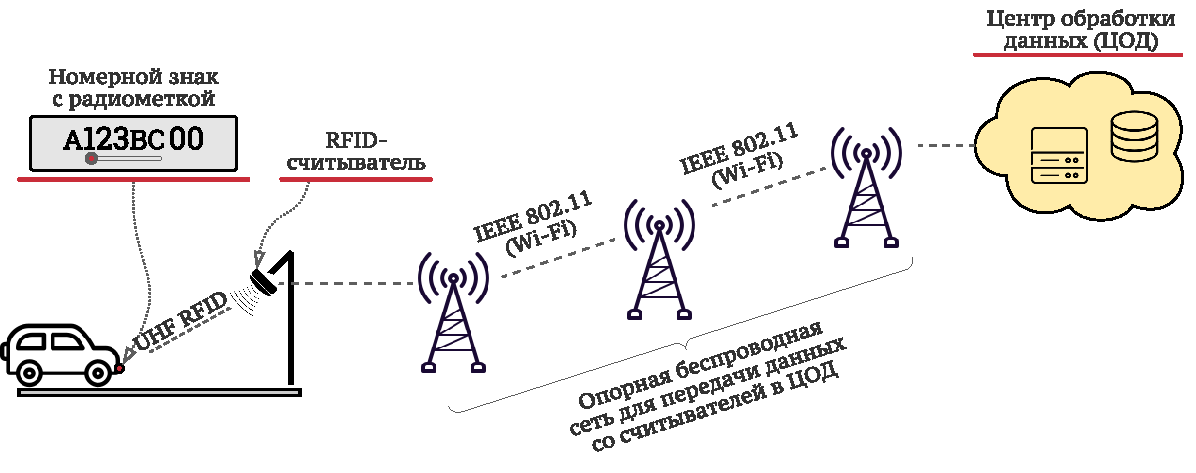
\includegraphics [scale=0.6] {chapter1/ch1_system_overview}
	\caption{Схема распределённой системы радиочастотной идентификации транспорта.}
	\label{fig:ch1_system_overview}
\end{figure}

Основными компонентами простейщей распределенной системы радиочастотной идентификации транспорта являются:

\begin{itemize}
    \item{\textbf{RFID-метки} (\textbf{транспондеры)}: устройства, которыми оснащаются транспортные средства. Их назначение "--- передача записанного идентификатора считывателям. В зависимости от используемой технологии, могут быть активными или пассивными, то есть иметь или нет свой источник питания. Подробнее принцип работы меток стандарта EPC Class 1 Gen. 2 (ISO 18000-6C) описан в разделе~\ref{sec:ch1_rfid}.}
    \item{\textbf{RFID-считыватели}: активные устройства, осуществляющие чтение идентификаторов меток и их передачу в центр обработки данных.}
    \item{\textbf{Опорная сеть}: используется для передачи данных о метках от считывателей в центр обработки данных, а также для доступа администраторов к считывателям для их настройки, обслуживания и мониторинга.}
    \item{\textbf{Центр обработки данных} (\textbf{ЦОД}): включает информационную систему, в которой собираются данные о прочитанных метках и состоянии работы считывателей.}
\end{itemize}

В качестве примера можно привести системы для бесконтактного сбора оплаты проезда на автодорогах, например "--- на участках трасс М-4 <<Дон>>, М-1 <<Беларусь>> и Центральной кольцевой автодороге (ЦКАД). В некоторых странах (например, в Чили, ЮАР, Азербайджане) проводились эксперименты по более масштабному внедрению RFID, для регистрации всех или определенной группы автомобилей. Подобный эксперимент проводился и в России, в республике Татарстан, его результаты будут более подробно рассмотрены в настоящей работе.

Для получения данных о проезжающем транспортном средстве оно должно быть оснащено одной или несколькими RFID-метками, причем выбранная технология радиочастотной идентификации должна обеспечивать чтение метки на расстоянии 10--20 метров. Одной из наиболее подходящих технологий RFID, отвечающих этому требованию, является СВЧ-RFID стандарта EPC Class 1 Generation 2~\cite{StdGen2}, работающая в диапазоне 860--920 МГц. В частности, эта технология была использована в эксперименте, проведенном в городе Казань. В качестве альтернативы также можно использовать активные метки, или технологию DSRC, которая используется на уже упомянутых платных дорогах М-1, М-4 и ЦКАД.

%\subtodo{Добавить ссылки на DSRC и активные RFID}

Для передачи информации о считанных метках RFID-считыватели должны быть подключены к центрам обработки данных. Возможны три пути решения этой задачи: подключение к существующей проводной или беспроводной сети, коммутационное оборудование которой находится вблизи точек размещения считывателей; использование сотовой сети; построение отдельной сети для подключения считывателей. Использование существующих сетей оказывается не всегда возможным, особенно при развертывании системы за пределами крупных населённых пунктов. Кроме того, сети могут быть перегружены (например, если они уже используются для передачи данных с городских камер видеонаблюдения). Из-за ограниченности покрытия использование сотовой сети также не всегда возможно. В качестве примера, в настоящем исследовании будем рассматривать построение отдельной беспроводной сети. Как будет показано, для работы системы не нужно высокоскоростных каналов, и для подключения большого количества считывателей (порядка нескольких сотен) достаточно многошаговой сети, построенной на основе технологии IEEE 802.11g, оборудование которой очень недорогое и позволяет строить беспроводные соединения на расстояниях до нескольких десятков километров.

В центре обработки данных должна собираться как информация о зарегистрированных считывателями метках, так и о состоянии работы оборудования. Если в состав системы входят камеры, радары и прочее оборудование, в информационном центре можно объединять данные, полученные от различных источников. Например, объединяя результаты идентификации номерных знаков по фото с данными, полученными от считывателей, можно существенно повысить достоверность распознавания транспортного средства в условиях плохой видимости. Возможна интеграция и с системами приема оплаты или с базами розыска угнанных машин.

\begin{table}[ht!]
    \renewcommand{\arraystretch}{1.3}
    \caption{Технологии, использованные в распределённой системе радиочастотной идентификации транспорта.}
    \label{table:ch1_technologies}
	\begin{tabular}{ |p{0.17\linewidth}|p{0.26\linewidth}|p{0.47\linewidth}| }\hline
		Компонент & Технология & Комментарии\\\hline\hline
		Метки & EPC Class 1 Gen. 2 & Пассивные метки в номерных знаках или на стикерах под лобовым стеклом.\\\hline
		Считыватели & EPC Class 1 Gen. 2 & RFID-считыватели устанавливаются над дорогой, поддерживают до четырх антенн и подключаются к сети.\\\hline
		Опорная сеть & IEEE 802.11 & Многошаговая беспроводная сеть с каналами, в которых используется схема доступа CSMA/CA.\\\hline
		ЦОД &  & Различное программное обеспечение для получения, сохранения и анализа данных о метках.\\\hline
	\end{tabular}

\end{table}

В ходе исследования, результаты которого приводятся в настоящей диссертационной работе, предполагалось, что для реализации распределённой системы радиочастотной идентификации транспорта используются технологии, описанные в табл.~\ref{table:ch1_technologies}.


% Следует оговориться, что в современных беспроводных сетях IEEE 802.11 используются гораздо более сложные и эффективные механизмы, нежели DCF, описываемый и исследуемый в настоящей работе; вместе с тем, механизм DCF гораздо проще для исследования, и, как будет показано в последующих главах, его вполне достаточно для эффективной реализации системы передачи данных со многих считывателей, что, вместе с низкой ценой соответствующего оборудования, делает его выбор вполне обоснованным для практической реализации.

% Технология радиочастотной идентификации далее рассматривается гораздо подробнее, чем протоколы передачи данных по беспроводным каналам. Это связано с тем, что вероятность идентификации движущихся меток, которая исследуется в следующих главах, существенно зависит от множества параметров протокола EPC Class 1 Generation 2. В то же время, при исследовании задержек в передаче данных по беспроводным каналам нас главным образом будет интересовать длительность обслуживания, в корректном моделировании которой заключается основная сложность работы, поэтому при описании протокола IEEEE 802.11 DCF мы сделаем акцент именно на временных аспектах работы и на механизме борьбы с коллизиями, игнорируя особенности кодирования и модуляции, а также прочие части протокола.




\section{Постановка задач исследования}\label{sec:ch1_problems}

При проектировании и построении распределённой системы радиочастотной идентификации транспорта возникает целый ряд задач, относящихся как непосредственно к идентификации транспорта, так и к организации связи между считывателями и центром обработки данных. Рассмотрим подробнее задачи, решению которых посвящена диссертационная работа.

\subsection{Исследование эффективности радиочастотной идентификации мобильных меток}

Критерием работоспособности системы является процент успешно распознанных транспортных средств. Задача осложняется тем, что метки могут двигаться с высокой скоростью (порядка 100--150~км/ч), а время, доступное для их чтения, крайне ограничено, так как считыватель может получить данные от метки лишь на небольшом расстоянии, порядка десяти метров. При различных настройках протокола EPC Class 1 Gen. 2 скорость обмена данными с меткой и вероятность успешной передачи сообщений могут меняться в очень широких пределах. Дополнительную сложность задаче придают многолучевое распространения сигналов между считывателем и меткой (как минимум, присутствие отраженного от дороги луча), наличие эффекта Доплера, а также использование метода обратного рассеяния для передачи ответов меток. Для решения задачи оценки работы системы радиочастотной идентификации удобно использовать методы имитационного моделирования, позволяющие учесть как параметры протокола, так и особенности распространения сигналов.

Отдельные аспекты работы считывателей можно исследовать с помощью методов теории случайных процессов. Хотя такой подход затрудняет учет всего объема факторов, влияющих на производительность системы, он позволяет более детально изучить отдельные закономерности, в частности "--- влияние периодических отключений питания и изменений подмножеств опрашиваемых меток на вероятность успешной идентификации. Для построения аналитической модели работы протокола нужно формально описать компоненты, определяющие состояние системы, а также формализовать операции, которые считыватель может осуществлять с метками. После этого можно исследовать свойства этих операций и найти способы получения оценки успешного чтения меток.

Таким образом, для исследования эффективности системы радиочастотной идентификации автомобилей нужно решить следующие задачи:

\begin{enumerate}
    \item Выявить факторы, влияющие на вероятность успешной идентификации мобильной RFID-метки.
    \item Построить формальную математическую модель системы радиочастотной идентификации, исследовать свойства операций, осуществляемых считывателем над множеством мобильных меток.
    \item Разработать аналитические и имитаицонные модели для получения оценки вероятности идентификации мобильных RFID-меток.
    \item Определить параметры протокола и настройки считывателей, при которых доля успешно идентифицированных автомобилей с RFID-метками оказывается не ниже 90\%.
\end{enumerate}

Решению этих задач посвящены главы 2 и 3 диссертации.



\subsection{Анализ производительности опорной сети}

Для работы некоторых приложений важно обеспечить быструю передачу информации о прочитанных метках в центр обработки данных. Например, это необходимо для реализации бесконтактной оплаты проезда или для поиска угнанных транспортных средств. Для анализа межконцевых задержек можно использовать как имитационное моделирование, так и аналитические модели, построенные на базе теории массового обслуживания.

Модели открытых тандемных сетей массового обслуживания хорошо известны и исследованы. Основная сложность их применения к задаче поиска межконецвых задержек пакетов, передаваемых в многошаговых сетях, заключается в выборе адекватных распределений интервалов между поступлениями пакетов в сеть и распределений длительности передачи пакетов по каналам связи. Как отмечалось ранее, в этом исследовании предполагается, что опорная сеть строится на базе беспроводных линий связи с каналами CSMA/CA.

В диссертационном исследовании предполагается, что для моделирования каналов связи используются системы массового обслуживания $MAP/PH/1/N$, в которых интервалы между поступлениями пакетов в сеть моделируются марковскими случайными потоками (MAP), время обслуживания пакетов имеет распределение фазового типа (PH), а размер очереди ограничен сверху. Получение численных характеристик открытых сетей $MAP/PH/1/N \rightarrow \bullet/PH/1/N \rightarrow \dots \rightarrow \bullet/PH/1/N$ осложняется экспоненциальным ростом проблемы при увеличении числа узлов в сети, и отдельной задачей является поиск эффективных способов получения численных оценок таких сетей.

Для оценки производительности опорной сети в диссертации решаются следующие задачи:

\begin{enumerate}
    \item Поиск PH-распределений, адекватно моделирующих время обслуживания в беспроводных сетях с каналами CSMA/CA.
    \item Оценка возможности использования методов редукции пространства состояний для получения численных оценок межконцевых задержек в открытых тандемных сетях массового обслуживания типа с узлами $MAP/PH/1/N$.
    \item Получение численных оценок межконецвых задержек для многошаговой беспроводной сети с помощью аналитического и имитационного моделирования.
    \item Оценка максимального количества считывателей, одновременно использующих беспроводную опорную сеть, с помощью имитационного и стендового моделирования.
\end{enumerate}

Решению этих задач посвящена глава 4 диссертации.


\subsection{Экспериментальная реализация системы}

Для того, чтобы исследовать работоспособность системы радиочастотной идентификации автомобилей, были разработаны экспериментальные RFID-считыватели, распределенная система управления считывателями и программное обеспечение для центров обработки данных. Разработанный программно-аппаратный комплекс проходил испытания в трех экспериментах. Первый эксперимент прошел в 2014--2015 годах в городе Казань. Тогда метками были оснащены около 750 автобусов, в двух точках города установлены RFID-считыватели, информация с которых передавалась в центр обработки данных в ГИБДД. За несколько зимних месяцев была собрана статистика, вероятность идентификации составила 92--95~\%. Следующий эксперимент проходил в 2020 году также в Казани, его целью была проверка системы при идентификации автомобилей, движущихся со скоростями до 170~км/ч и совершающих различные маневры. Третий эксперимент начался летом 2021 года на ЦКАД, его цель "--- проверка применимости системы для сбора данных для оплаты проезда. Первые два эксперимента завершились успешно, последний эксперимент на момент написания диссертационной работы еще не завершен.

При разработке программного обеспечения RFID-считывателей требовалось обеспечить его высокую надежность, быстродействие, а также гибкость. В частности, было принято решение разделить потоки данных и управления (сигнализации) так, чтобы, с одной стороны, сделать невозможным изменение параметров работы считывателя каким-либо образом, кроме как через административный интерфейс, а с другой стороны "--- упростить подключение внешних клиентов для получения потоков считанных меток. Программное обеспечение было спроектировано таким образом, чтобы можно было в быстро заменить радиомодули RFID-считывателей без изменения кода остальных компонентов, а также обеспечить возможность выноса части компонентов за пределы считывателя.

В состав разработанного программного обеспечения входит управляющий модуль (супервайзер), адаптеры радиомодулей, интерфейсы управления (веб-интерфейс, интерфейс командной строки), а также модули для приема и обработки потоков данных о прочитанных метках. Все программное обеспечение, за исключением веб-интерфейса, было реализовано на языках C и C++.

Для экспериментального исследования производительности системы радиочастотной идентификации были решены следующие задачи:

\begin{enumerate}
	\item Разработка архитектуры распределённой системы управления RFID-считывателями и протоколов связи между компонентами системы.
	\item Программная реализация распределённой системы управления и разработка программного обеспечения для приема, обработки и записи данных о прочитанных метках.
	\item Проведение экспериментальных исследований и получение оценки вероятности успешной идентификации автомобилей при различных скоростях движения, маневрах, погодных условиях.
\end{enumerate}

Решению этих задач посвящена глава 5 диссертации.




\section{Радиочастотная идентификация транспортных средств}\label{sec:ch1_rfid}

Технология радиочастотной идентификации (RFID) является альтернативой для традиционной идентификации номеров транспортных средств по фото. Для использования этой технологии автомобили оснащаются радиометками, а в точках контроля размещаются считыватели. Когда метка проезжает мимо считывателя, она передает свой идентификатор, по которому определяется номер автомобиля. К преимуществам этой технологии относится относительно низкая стоимость оборудования, низкие требования к пропускной способности каналов связи, отсутствие необходимости в частом обслуживании и слабая зависимость от погодных условий.

Существует несколько различных технологий радиочастотной идентификации. В \textbf{активных} системах используются метки, обладающие собственным источником питания. Часто такие системы работают в диапазоне 2.4 ГГц и могут быть основаны, например, на технологиях IEEE 802.11 (WiFi) или ZigBee. Можно выделить технологию DSRC (Dedicated Short-Range Communication), которая часто используется в системах оплаты проезда по автомагистралям, в том числе и в России. Дальность действия считывателя в системах с активными метками может достигать десятков или даже сотен метров, но метки достаточно громоздки и дорогостоящи.

К другому классу относятся \textbf{пассивные} системы, в которых метки не обладают собственными источниками энергии. Для работы и передачи данных метки в таких системах используют энергию, получаемую из электромагнитного поля, создаваемого считывателем. RFID-системы LF-диапазона (125 "--- 134 кГц, ISO/IEC 18000-2) характеризуются малым расстоянием идентификации (порядка нескольких сантиметров) и используются, например, для чипирования животных. Системы HF-диапазона (13,56 МГц, стандарты ISO/IEC 18000-3, ISO/IEC 15693, ISO/IEC 14443 A,B) очень широко распространены в области электронной оплаты (например, оплата проезда на общественном транспорте) и контроля доступа, характеризуются низкой стоимостью и дальностью порядка нескольких миллиметров или сантиметров. Системы UHF-диапазона (860 "--- 960 МГц, ISO/IEC 18000-6C, EPC Gen-2) работают на расстояниях до 15--20 метров и используются в логистике, торговле, контроле доступа и на производствах. Кроме того, метки UHF-диапазона иногда оснащаются собственным источником питания, который может использоваться для работы встроенного сенсора. В этом случае метка может передавать результаты измерений, полученные от сенсора, а питание также может использоваться для усиления отражаемых сигналов. Такие метки называются полупассивными или полуактивными.


\subsection{Стандарт EPC Class 1 Generation 2}

Стандарт EPC Class 1 Generation 2 (ISO/IEC 18000-6C)~\cite{StdGen2} описывает физический (PHY) и канальный (MAC) уровни системы радиочастотной идентификации пассивных и полупассивных меток. На физическом уровне стандарт описывает способы модуляции и кодирования сигналов, передаваемых считывателями и метками. На канальном уровне описывается протокол обмена данными между считывателем и метками. Этот протокол основан на протоколе Slotted ALOHA \cite{Abramson1970, Roberts1975}, позволяет бороться с коллизиями при нахождении нескольких меток в зоне считывателя, а также содержит средства для чтения и записи данных на метки.

Поскольку пассивные метки не имеют собственного источника питания, счиытватель постоянно создает электромагнитное поле, которое используется метками для получения энергии. Необходимо отметить, что в действительности считыватель может периодически выключаться, обеспечивая тем самым меткам возможность сбросить некоторые регистры и флаги, о которых будет сказано позднее. В то время, когда считыватель не осуществляет передачу своих команд, он генерирует синусоидальный сигнал (Constant Wave, CW), который метки используют в качестве несущей "--- для передачи ответов метки модулируют отражаемый ими сигнал CW, полученный от считывателя, изменением своего коэффициента отражения (т.е. передача данных от меток ведётся методом обратного рассеяния).

Метки не могут сами инициировать обмен данными со считывателем, они всегда передают свои сообщения в ответ на получаемые от считывателя команды. Стандарт допускает следующие основные действия с меткой: инвентаризацию, чтение, запись и блокирование памяти, а также уничтожение метки. Инвентаризация "--- это опрос меток, в ходе которого они передают считывателю свои идентификаторы EPCID и выполняют другие операции, которые может запросить считыватель.  Блокирование памяти означает, что считыватель впоследствии не сможет записать эту область памяти. Наконец, операция уничтожения метки приводит к тому, что в будущем метка никогда не будет участвовать в инвентаризации. Протокол определяет и другие операции, включая средства для защиты доступа к данным. Производители могут реализовать дополнительные операции на своих метках. В рамках настоящей работы интерес будут представлять только инвентаризация и чтение памяти.


\subsubsection{Логическая структура памяти метки}

Каждая метка включает в себя четыре банка памяти (см. рис. \ref{fig:rfid-memory-banks}): EPC, TID, зарезервированную память (Reserved) и пользовательскую память (User).

\begin{figure}[ht]
  \centering
  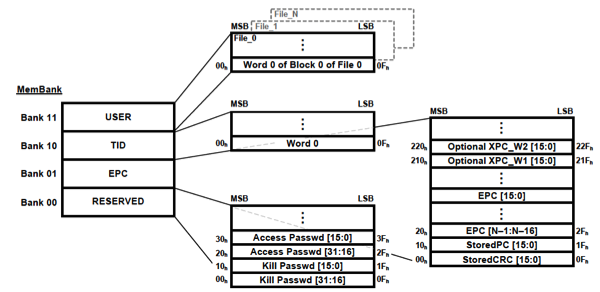
\includegraphics [scale=0.6] {chapter1/ch1_banks.png}
  \caption{Логическая структура памяти метки \cite{std_gen2}}
  \label{fig:rfid-memory-banks}
\end{figure}

Банк EPC содержит код EPC (Electronic Product Code), контрольную сумму (StoredCRC) и служебную информацию (PC, Protocol Control), в которой хранятся данные о длине поля EPC, доступности пользовательской памяти и прочую информацию. Объем памяти в поле EPC может меняться от метки к метке, распространненым значением является 96 бит. Чтобы не путать название банка памяти и значение EPC, значение в дальнейшем будем называть EPCID.

Банк Reserved хранит пароли для блокирования и уничтожения меток, если метка поддерживает соответствующие операции.

Банк TID хранит данные о производителе и модели метки, а также ее уникальный идентификатор. Главная особенность банка TID "--- фабричная защита от изменений значения, записанного при производстве метки, поэтому его удобно использовать в задаче надежной идентификации объектов. Первые 8 бит TID содержат идентификатор класса, который может быть равен либо $\text{E0}_\text{h}$, либо $\text{E2}_\text{h}$. Если идентификатор класса равен $\text{E0}_\text{h}$, то длина банка равна 64 битам, второй октет содержит идентификатор производителя, а последние 48 бит содержат серийный номер метки. Такие метки производства NXP использовались в эксперименте в Казани в 2014 году. Структура банка TID для класса $\text{E2}_\text{h}$ более сложная, а его размер "--- больше. Следюущие после первого октета три бита "--- служебные флаги, после них "--- 9-битный идентификатор производителя MDID (Mask Designer Identifier), далее 12-битный номер модели и уже после него уникальный номер метки. Например, метки производства АО <<Микрон>>, которые использовались в экспериментах 2020-го и 2021-го года, имеют класс $\text{E2}_\text{h}$ и содержат 96-битные значения.

Банк пользовательской памяти может иметь достаточно большой объем (порядка 512 бит) и используется для хранения дополнительных данных (например, более подробной информации о маркированном предмете).


\subsubsection{Физический уровень}

При передаче данных от считывателя к меткам используется амплитудную модуляцию DSB-ASK, SSB-ASK или PR-ASK. Для кодирования используется схема PIE (Pulse Interval Encoding), в которой нули и единицы кодируются символами \texttt{data-0} и \texttt{data-1} различной длины (см. рис.~\ref{fig:rfid-pie-symbols}).

\begin{figure}[ht]
  \centering
  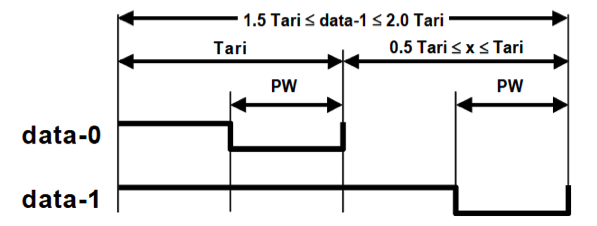
\includegraphics [scale=0.45] {chapter1/ch1_pie_symbols.png}
  \caption{Символы в кодировке PIE \cite{std_gen2}}
  \label{fig:rfid-pie-symbols}
\end{figure}

Перед передачей каждой команды считыватель передает синхронизирующую последовательность (преамбулу), символы в которой также кодируются с помощью PIE. Стандарт определяет два вида преамбул (см. рис.~\ref{fig:rfid-reader-preambles}): длинную (называемую в стандарте преамбулой) и короткую (называемую синхронизацией кадра).

\begin{figure}[ht]
  \centering
  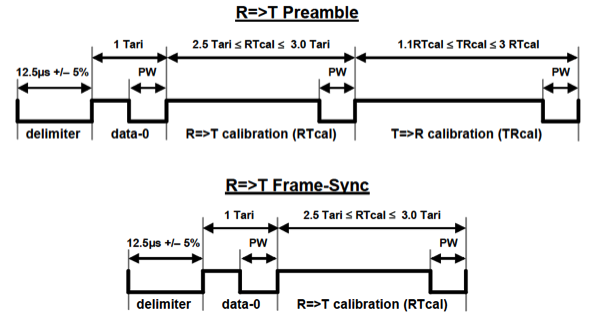
\includegraphics [scale=0.45] {chapter1/ch1_reader_preambles.png}
  \caption{Преамбулы кадров считывателя \cite{std_gen2}}
  \label{fig:rfid-reader-preambles}
\end{figure}

Преамбулы содержат следующие символы:

\begin{itemize}
	\item \texttt{delimiter}: символ-разделитель, имеющий фиксированную длину 12.5 мкс;
	\item \texttt{Tari}: символ, равный по длительности \texttt{data-0};
	\item \texttt{RTcal} (Reader-Tag Calibration): символ, равный сумме длительностей нуля и единицы. Метки используют его для того, чтобы различать нули и единицы: если информационный символ короче половины \texttt{RTcal}, то он декодируется как ноль, в противном случае "--- как единица;
	\item \texttt{TRcal} (Tag-Reader Calibration): символ, использующийся меткой для расчет скорости передачи ее ответов.
\end{itemize}

Длинная преамбула отличается от короткой наличием символа \texttt{TRcal} и передается перед первой командой \texttt{Query}, с которой считыватель начинает опрос меток. Так как метка, не получившая \texttt{Query}, все равно не сможет участвовать в опросе, передавать \texttt{TRcal} в последующих кадрах не имеет смысла и используется короткая преамбула, содержащая только ту информацию, которая нужна метке для успешного декодирования команды.

Необходимо заметить, что из-за использования кодирования PIE длительность кадров, передаваемых считывателем, зависит не только от параметров \texttt{Tari} и \texttt{RTcal}, но и от содержания передаваемых команд, поэтому для точного моделирования протокола необходимо учитывать результат кодирования команд.

Метка передает свой ответ, модулируя несущую, полученную от считывателя. Метка может использовать амплитудную (ASK) или фазовую (PSK) модуляцию. В качестве схемы кодирования используется либо код FM0, либо коды Миллера с 2, 4 или 8 символами на бит. Все схемы кодирования, поддерживаемые метками, имеют память, то есть вид символа, кодирующего следующий бит, определяется предыдущим битом. Перед передачей ответа метка передаёт преамбулу, которая может быть обычной или расширенной. Короткая преамбула равна по длительности 6 битам для кода FM0 и 10 битам для кодов Миллера, а расширенная - 18 и 22 битам соответственно. Кроме того, после каждого ответа метки следует символ, не кодирующий ни ноль, ни единицу.

Для вычисления скорости передачи символов метка вычисляет величину BLF (Backscatter Link Frequency) по следующей формуле:

$$
\text{BLF} = \frac{\text{DR}}{\text{TRcal}},
$$

где \texttt{DR} (Divide Ratio) - величина, передаваемая в команде \texttt{Query}, и принимающая одно из двух значений: 8 или 64/3. Для вычисления битовой скорости необходимо разделить \texttt{BLF} на число символов на бит в используемом меткой методе кодирования (M=1,2,4,8). В отличие от считывателей, использующих PIE, все биты в ответах меток имеют одинаковую длительность, поэтому их содержание не оказывает влияния на длительность передачи ответов.




\subsubsection{Канальный уровень}

Протокол доступа к каналу, описываемый в стандарте \cite{std_gen2}, основан на протоколе Framed Slotted ALOHA \cite{Roberts1975, Abramson1970}. Все время работы разбито на \textbf{раунды} (см. рис. \ref{fig:rfid-round-examples}), которые начинаются передачей считывателем команды \texttt{Query}, которая, среди прочего, несет в себе параметр \texttt{Q}, использующийся метками для расчета количества слотов в раунда как $2^\text{Q}$. Получив \texttt{Query}, метка вычисляет количество слотов и вычисляет случайный номер слота для передачи своего ответа, в полученное значение устанавливается счетчик \textit{SN}. При последующем получении команд \texttt{QueryRep} метка уменьшает значение этого счетчика, и когда он доходит до 0, генерирует и передает случайное 16-битное число (слово RN16). Считыватель, получив это случайное число, пересылает его в команде \texttt{ACK}, в ответ на который метка пересылает свой EPC (точнее, вместе с EPC пересылается часть PC и StoredCRC).

\begin{figure}[ht]
  \centering
   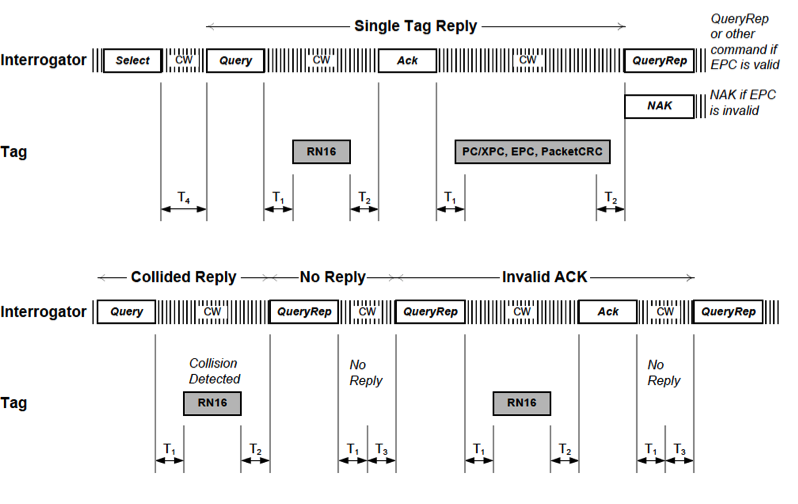
\includegraphics [scale=0.45] {chapter1/ch1_round_examples}
  \caption{Пример опроса меток \cite{std_gen2}}
  \label{fig:rfid-round-examples}
\end{figure}

Стандарт определяет границы интервалов, которые должны пройти между последовательными командами и ответами:

\begin{itemize}
	\item $T_1$: минимальное время между концом последнего символа команды и первым символом преамбулы ответа;
	\item $T_2$: минимальное время между окончанием последнего (псевдо-) бита ответа метки и первым символом преамбулы команды считывателя;
	\item $T_3$: минимальный интервал между окончанием $T_1$ и следующей командой считывателя.
\end{itemize}

\begin{figure}[ht]
  \centering
  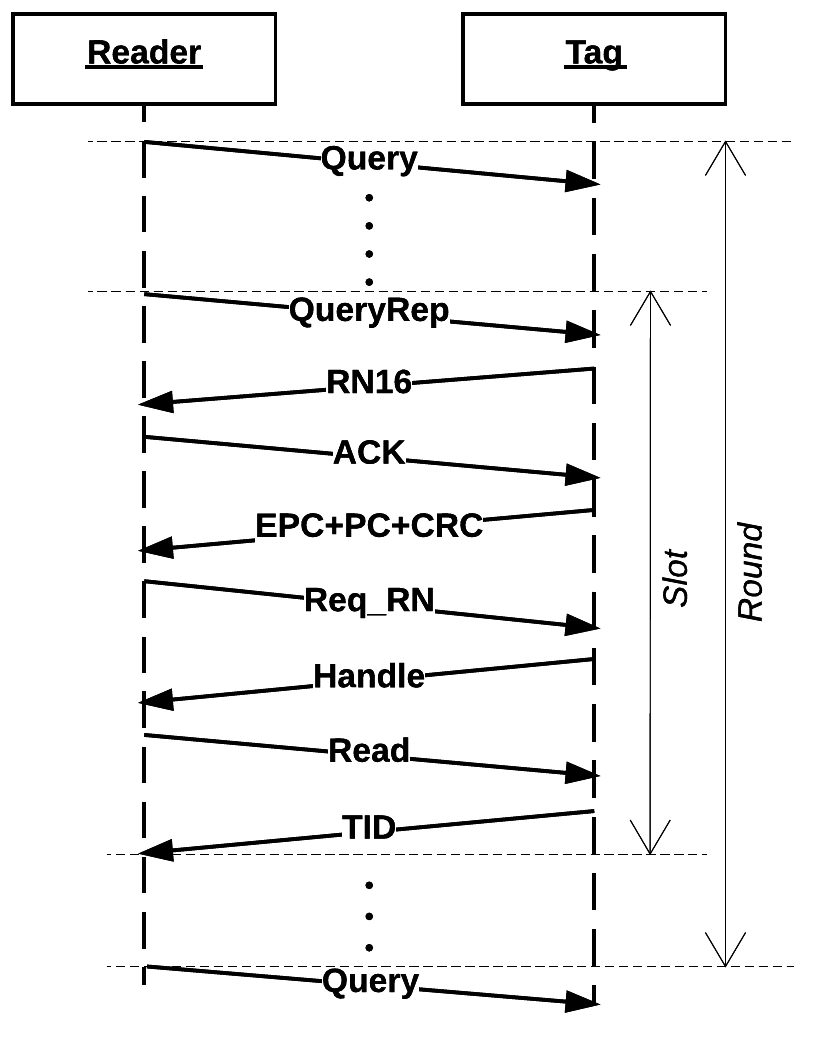
\includegraphics [scale=0.3] {chapter1/ch1_read_sequence_example}
  \caption{Обмен сообщениями для чтения банка памяти}
  \label{fig:rfid-read-sequence-example}
\end{figure}

Для того, чтобы получить значение из банка памяти (например, прочитать \texttt{TID}), считыватель, после получения ответа от метки с её \texttt{EPCID}, передает команду \texttt{Req\_RN}, в ответ на которую метка генерирует новое случайное число и передает его считывателю (\texttt{Handle}). Получив \texttt{Handle}, считыватель передает команду чтения \texttt{Read}, в которой указывает банк памяти, смещение с его начала и количество слов. В ответ метка пересылает данные из этого банка, см. рис. \ref{fig:rfid-read-sequence-example}.



\subsubsection{Сессии}

Сессии позволяют разграничить множество окружающих считыватель меток. Каждая метка должна поддерживать четыре сессии \texttt{S0}, \texttt{S1}, \texttt{S2} и \texttt{S3}; для каждой сессии метка имеет отдельный флаг, значения которого в стандарте обозначаются как $A$ и $B$.

В команде \texttt{Query} считыватель указывает, с какой сессией работает в начинающемся раунде, и какое значение флага сессии должно быть у меток, которые могут участвовать в опросе. Правила изменения значений флагов метками таковы, что после передачи \texttt{EPCID} метка, получив команду \texttt{Query}/\texttt{QueryRep}/\texttt{QueryAdjust}, должна инвертировать его. Таким образом, в последующих раундах, опрос в которых будет производиться в той же сессии и с тем же флагом, метка участвовать не будет. Если считыватель не смог получить \texttt{EPCID}, он может передать команду \texttt{NAK}, из-за чего метка не изменит флага и сможет участвовать в последующих раундах.

Сессии различаются по требованиям ко времени сохранения значения флага при потере питания, а также к начальным значениям флагов:

\begin{itemize}
	\item Флаг сессии \texttt{S0} всегда инициализируется в значение $A$;
	\item Флаг сессии \texttt{S1} сбрасывается в значение $A$ при включении метки, если со времени его изменения прошло не менее интервала, значение которого может варьироваться от 0.5 с до 5 с. Значение также сбрасывается в том случае, если метка не выключалась и со времени последнего изменения прошло слишком много времени;
	\item Флаги сессий \texttt{S2} и \texttt{S3} должны сбрасываться в $A$, если с момента выключения метки прошло не менее 2 с.
\end{itemize}

Таким образом, использование сессий \texttt{S2} и \texttt{S3} может предотвратить изменение флага в случае краткосрочной потери меткой энергии, а сессия \texttt{S0} сбрасывается всякий раз, когда метка выключается.

Как будет показано далее, выбор сессии и сценария опроса (всегда ли опрашивать метки по значению флага $A$ или чередовать опросы по $A$ и по $B$) оказывает существенное влияние на вероятность успешной идентификации метки.



\subsection{Исследования производительности UHF RFID}

Протокол, лежащий в основе канального уровня стандарта EPC Gen-2 \cite{std_gen2}, "--- Framed Slotted ALOHA. Исходный протокол ALOHA был представлен в работе \cite{Roberts1975}. В этой же работе, на основе предположения о пуассоновском потоке передаваемых пакетов, была получена оценка пиковой пропускной способности сети как $1/(2e) \approx 0,186$. Позднее в работе \cite{Abramson1970} был описан способ повышения пропускной способности в два раза за счет разбиения времени на слоты (Slotted ALOHA).

Значительное число работ посвящено анализу производительности систем радиочастотной идентификации. Авторы пользуются эмпирическими методами \cite{Buettner2008}, используют аппарат марковских случайных процессов как с идеальным каналом \cite{Wang2009, Vahedi2012, Vales-Alonso2009, Vales-Alonso2011, Qiaoling2007}, так и с каналом с ошибками \cite{DiMarco2014}, а также используют иные аналитические подходы для анализа производительности \cite{Ahmed2016, Yan2014, Jeon2009}. В ряде работ также сравнивается производительность протокола Frame Slotted ALOHA с альтернативными протоколами и расширениями \cite{Vahedi2014, LaPorta2011}.

В качестве примера эмпирического анализа производительности системы радиочастотной анализа можно привести работу M. Buettner \cite{Buettner2008}. В этой работе исследуются факторы, влияющие на производительность чтения стационарных меток. Авторы используют две различные модели считывателей и анализатор, разработанный на базе USRP (Universal Software Radio Peripheral) и GNU Radio. В статье рассматриваются следующие вопросы: насколько хорошо работают на практике коммерческие считыватели, какаие параметры протокола влияют на понижение производительности, из-за чего метки теряются при чтении и каким образом можно увеличить производительность системы. На основе сделанного исследования авторы делают следующие выводы: размер множества меток влияет на производительность системы обратно пропорционально, т.к. при увеличении числа меток снижаются служебные расходы в пересчете на метку; более медленные и надёжные способы кодирования ответов меток тем эффективнее, чем больше расстояние до считывателя; существенное влияние оказывает окружение по причине многолучевого характера распространения сигнала; из-за ошибок при передаче кадров растет как общая длительность раундов, так и её вариация; команды \texttt{ACK}, \texttt{Query} / \texttt{QueryRep} занимают большую долю общего времени работы протокола, особенно если \texttt{ACK} повторно пересылается при возникновении ошибок; ошибки в передаче кадров ведут как к увеличению длительности раундов, так и к потере меток; более низкие скорости канала от считывателя к меткам ведут к понижению числа раундов, необходимых для чтения; основной источник потерь "--- многолучевое распространение сигнала, зависящее от частоты. На основе проведенного исследования авторы дают следующие рекомендации, направленные на повышение производительности системы радиочастотной идентификации: сокращать интервалы ожидания ответов от меток; как можно чаще переключать каналы считывателя (вплоть до изменения на старте каждого раунда) для того, чтобы менять картину распространения сигнала; не пересылать повторно команды \texttt{ACK} при потере ответа от метки (лучше выключиться и попробовать в следующем раунде или использовать иную стратегию опроса); между раундами менять настройки физического уровня "--- например, в первом раунде использовать самые быстрые настройки для чтения как можно большего числа меток, и постепенно переходить к более надежным.

Задача идентификации транспорта является одним из основных применений RFID. Первые системы сбора платы за проезд, использующие RFID, появились в США в 1991 году \cite{Landt2001}. Использование RFID в системах контроля доступа, сбора платы за проезд и прочих системах исследовались в работах \cite{Karmakar2013, Blythe99, Khan2011, Yoon2008, Fawzi2011, Tseng2007}.

Также значительное число работ было посвящено имитационному моделированию систем UHF RFID \cite{Floerkemeier09, Arnitz2009, Zhang2010}. Так, в работе \cite{Floerkemeier09} была предложена модель JiST, реализованная на языке Java, в частности описывается дизайн системы моделирования, а также применение для различных сценариев. К сожалению, симулятор JiST давно не обновлялся и, судя по всему, в настоящее время практически не используется. В работе \cite{Arnitz2009} сделан фокус на особенности распространения сигналов, моделировании каналов передачи данных и прочих низкоуровневых особенностях RFID-системы, однако практически не учитываются аспекты верхнего (логического) уровня. Авторы работы \cite{Zhang2010} предлагают использовать комбинацию симулятора OMNeT++ для моделирования логики и MATLAB для моделирования физического уровня, в качестве примера рассматривают модель UHF RFID.

Для того, чтобы адекватно моделировать процесс обмена сообщениями, учитывая потери из-за ненадежности каналов связи между считывателем и меткой, требуется детально учитывать особенности распространения сигналов. Этот вопрос изучался в работах \cite{Dimitriou14, Azpilicueta16}. Обе работы предлагают модели распространения сигналов, основанные на технике трассировки лучей. Авторы работы \cite{Dimitriou14} рассматривают особенности распространения сигналов внутри помещений со множеством отражений, однако акцентируются на стационарных объектах и игнорируют эффект Доплера. В работе \cite{Azpilicueta16} авторы моделируют систему с движущимися транспортными средствами, однако не учитывают параметры логического уровня и сосредотачиваются на оценке энергетических параметров в сравнении с данными, полученными из эксперимента. Наконец, в работе \cite{Griffin09} предложена точная модель для расчёта бюджета соединений.








\section{Передача данных по беспроводным сетям}

Исторически, одним из первых методов доступа к каналу стал CSMA/CA, который был взят за основу уже в первых версиях стандарта IEEE 802.11. Базовый механизм доступа, описанный в этом стандарте и основанный на CSMA/CA, называется DCF (Distributed Coordination Function). Хотя современные версии стандарта используют гораздо более совершенные методы конкурентного доступа, позволяющие учитывать QoS, производить групповые передачи, подтверждать группы пакетов вместо отдельных, объединять каналы и пр., так или иначе в их основе лежит DCF. Ввиду своей простоты, мы будем использовать его в качестве модельного образца конкурентного доступа к каналу.

С другой стороны, в релейных беспроводных каналх связи практически отсутствует конкуренция: релейные станции располагаются в области прямой видимости, используют сильно направленные антенны, зачастую работают в лицензированных диапазонах частот. Хотя, безусловно, передача по таким линиям связи может быть менее надежной, чем по проводным каналам, она по своим свойствам оказывается гораздо ближе к передаче именно к проводным линиям связи. Для доступа к каналу в релейных сетях чаще всего используются методы, схожие с сетями Ethernet.

В настоящей работе мы будем рассматривать два модельных варианта доступа к каналу:

\begin{enumerate}
\item доступ без конкуренции для релейных каналов;
\item доступ с конкуренцией DCF для каналов стандарта IEEE 802.11.
\end{enumerate}

В обоих случаях мы делаем предположение об идеальности канала, то есть кадры, не вступающие друг с другом в коллизии, всегда успешно доставляется (Bit error rate, BER, равен нулю). В более общем случае, безусловно, желательно использовать более реалистичные модели канала.

\subsection{Метод доступа в радиорелейной сети}

\begin{figure}[h!]
   \centering
    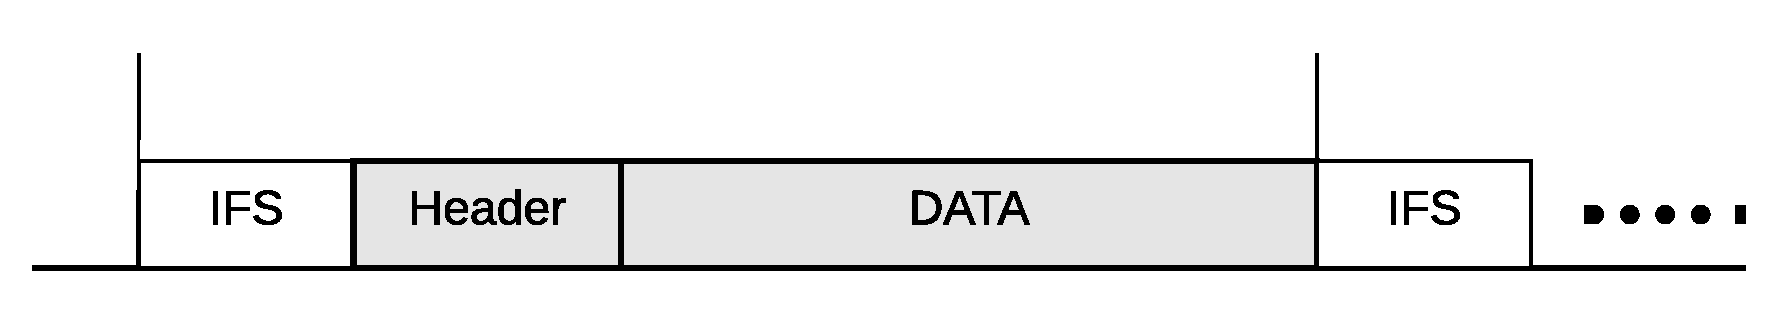
\includegraphics[width=0.5\textwidth]{chapter1/ch1_relay_channel}
	\caption{Организация доступа к каналу в релейной линии}
	\label{fig:relay}
\end{figure}

В качестве модельного примера доступа к каналу в радиорелейной линии, мы будем использовать очень простую схему без прослушивания канала в течение случайного времени. Схема доступа показана на рис.~\ref{fig:relay}: между последовательным кадрами станция ждет в течение фиксированного интервала IFS (Inter-Frame Space), после чего передает пакет, начиная с заголовков. Подтверждения успешности передачи не передаются. Предполагается, что используется частотный дуплекс, то есть станции линии используют две частоты для одновременной передачи и приема.

Здесь нужно сделать два уточнения. Во-первых, передача кадра всегда начинается с преамбулы, которая нужна приемнику для синхронизации с передатчиком. Мы не стали ее отдельно выделять, поскольку нас интересует лишь время, затрачиваемое станцией на передачу и, хотя передача прембулы также в него входит, с точки зрения оценки времени -- это лишь дополнительная константа, поэтому можно ее неявно ``включить'' в IFS или в заголовок. Во-вторых, в общем случае IFS необходимо ждать не всегда, а только при последовательной передаче несколько кадров. Хотя это несколько ускоряет передачу данных, если между пакетам передатчик освобождается на время, большее IFS, мы не учитываем это и считаем, что IFS необходимо ждать всегда перед (или после) передачи кадра. Это допущение обусловлено желанием использовать PH-распределение времени обслуживания; если же во временах обслуживания последовательных пакетов появляется зависимость, то необходимо использовать более сложные модели, например - MSP (Markovian Service Process), что выходит за рамки настоящей работы и предполагается исследовать в дальнейшем.



\subsection{Метод доступа в сети IEEE 802.11 DCF}

Метод доступа CSMA/CA и механизм DCF хорошо известны и подробно описаны в различных статьях и книгах (например, см. \cite{Bianchi2000}), а наиболее подробное описание можно найти в стандарте IEEE 802.11. Здесь мы вкратце опишем основы механимза.

Когда станции требуется передать новый пакет, в первую очередь она должна убедиться, что канал свободен. Если канал остается свободен в течение интервала DIFS (DCF Interframe Space), то станция выбирает случайное число слотов ожидания в интервале от 0 до CW-1 (CW - Contention Window). Значение CW при первой попытке передачи равняется CWmin. Каждый слот имеет фиксированную длительность $\sigma$. Если в течение выбранного числа слотов канал остается свободным, то станция начинает передачу. В противном случае, если канал стал занят в течение очередного слота, станция останавливает отсчет, ждет освобождения канала, прослушивает его еще в течение DIFS, и после этого возвращается к отсчету слотов. Если передача прошла успешно, принимающая станция должна после интеврала SIFS (Short Interframe Space, всегда короче DIFS) передать подтверждение ACK. Если подтверждение не было получено, передающая станция удваивает значение CW и повторяет попытку передачи. По достижении CW значения CWmax увличение окна прекращается. Механизм такого ожидания передачи называется \textit{backoff}. Возможные события при передаче показаны на рис.~\ref{fig:dcf}.

\begin{figure}[h!]
   \centering
    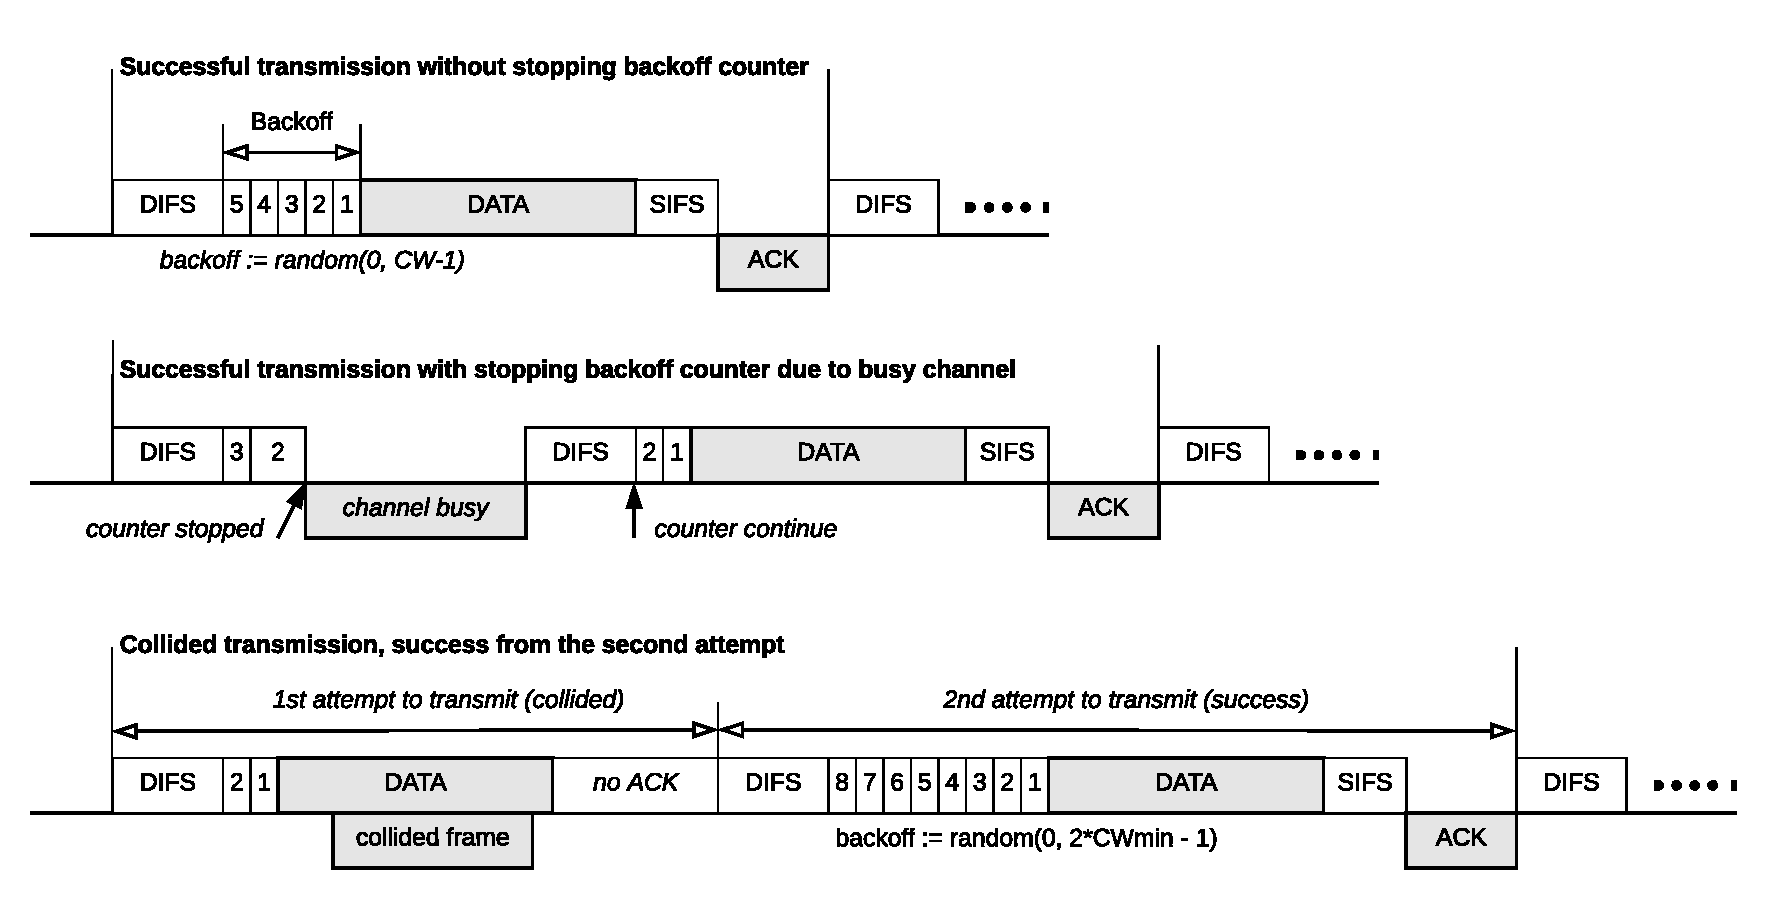
\includegraphics[width=0.9\textwidth]{chapter1/ch1_dcf_channel}
	\caption{Организация доступа к каналу при использовании простейшей версии механизма DCF}
	\label{fig:dcf}
\end{figure}

В действительности, механизм DCF имеет ряд дополнительных возможностей, позволяющих увеличить эффективность передачи. Во-первых, если передаваемые данные имеют достаточно большой размер, перед их передачей станция может отправить кадр RTS (Request to Send), в котором передается ожидаемое время занятости канала. В ответ на RTS получатель передает CTS (Clear to Send), которым подтверждает готовность вести прием. Этот механизм позволяет решить проблему скрытых станций. Кроме того, после успешной передачи станция может начать отсчет backoff и, если новый пакет придет от сетевого уровня до того, как отсчет закончится, ему потребуется ждать передачи меньше времени. Количество попыток передачи пакета ограничено, и при его достижении пакет, вообще говоря, отбрасывается как недоставленный. Стоит также отметить, что при передаче больших пакетов может использоваться дефрагментация, и отдельные фрагменты могут передаваться без дополнительных отсчетов backoff. В настоящей работе мы не станем учитывать эти механизмы, однако в дальнейшем их можно учесть для повышения точности моделирования. Что касается post-backoff и передачи группы кадров получившей доступ к каналу станцией (EDCA), для их адекватного учета нужно использовать более сложные методы описания времени передачи, например -- MSP.

\subsection{Параметры механизмов доступа к каналу в беспроводной сети}

В дальнейшем в настойщей работе будут использоваться значения параметров, приведенные в табл.~\ref{tab:ch1_channel_parameters}, если явно не указаны другие значения. Эти параметры в основном совпадают с параметрами из работы \cite{Bianchi2000}, что упрощает валидацию моделей. Вместе с тем, их можно легко изменить для анализа более высокоскоростных современных версий каналов IEEE 802.11. Также в таблице приведены параметры, используемые в релейных линиях, которые будут использоваться нами. Несложно видеть, что длительность IFS равняется DIFS, и мы не стали выделять отдельно преамбулу, поскольку в предположении о том, что канал идеален, она становится лишь дополнительной константой. Кроме этого, в таблице приведены параметры трафика, которые мы будем использовать при моделировании сети в ненагруженном режиме.

\begin{table}[h!]\begin{center}
\begin{tabular}{|c|c|c|c|}\hline
Параметр & Значение & Единицы & Модели\\ \hline\hline
Заголовок PHY & 128 & бит & DCF, РК\\ \hline
Заголовок MAC DATA & 272 & бит & DCF, РК \\ \hline
Кадр MAC ACK & 112 & бит & DCF \\ \hline
Слот ($\sigma$) & 50 & мкс. & DCF \\ \hline
IFS & 128 & мкс. & РК \\ \hline
DIFS & 128 & мкс. & DCF\\ \hline
SIFS & 28 & мкс. & DCF \\ \hline
CWmin & 16 & - & DCF \\ \hline
CWmax & 1024 & - & DCF \\ \hline
Скорость канала & 1000 & кбит/с & DCF, РК \\ \hline
Заголовок IP & 160 & бит & DCF, РК \\ \hline\hline
Средний размер данных ($\overline{\xi}$) & 9000 & бит & DCF, РК\\ \hline
Стандартное отклонение ($\sigma_\xi$) & 1688 & бит & DCF, РК\\ \hline
Трафик низкой интенсивности ($B_l$) & 1 & кбитсюс & DCF, РК \\ \hline
Трафик средней интенсивности ($B_m$) & 20 & кбит/с & DCF, РК\\ \hline
Трафик высокой интенсивности ($B_h$) & 150 & кбит/с & DCF, РК \\ \hline
\end{tabular}\caption{Параметры механизмов доступа к каналу и режимы передачи трафика, использованные при моделировании беспроводных сетей (РК "--- релейный канал).}\label{tab:ch1_channel_parameters}
\end{center}\end{table}



\subsection{Методы анализа производительности беспроводных каналов связи}

Из всех характеристик беспроводных каналов, в дальнейшем нас в первую очередь будет интересовать время, необходимое для передачи одного сообщения. Для оценки длительности передачи сообщений, а также для оценки пропускной способности канала часто используются марковские или полумарковские случайные процессы. В таких моделях состояние случайного процесса описывает состояние канала (например, <<канал занят, ждать ещё два слота>> или <<ведётся передача>>), и либо производится оценка доли времени, которое процесс находится в определенных состояниях, либо времени, нужного для попадания в некоторое состояние. Использованию марковских и полумарковских процессов для анализа производительности беспроводных сетей на основе CSMA/CA посвящено большое количество работ. Одной из ключевых работ в этой области является работа Bianchi \cite{Bianchi2000}, в которой была предложена марковская цепь, моделирующая работу станции сети IEEE 802.11 под управлением механизма доступа DCF. Состояния цепи соответствуют слотам ожидания backoff и попыткам передачи. Ключевым допущением модели является постоянство условной вероятности коллизии при передаче, а также насыщенный режим работы. С помощью предложенной цепи рассчитывается пропускная способность сети в насыщенном режиме. Полумарковские процессы также часто используются для описания работы беспроводной сети. Например, в работе \cite{Lauwens2010} предложен полумарковский процесс, моделирующий работу канального уровня сети IEEE 802.15.4-2006. Вместе с полумарковским процессом рассматривается процесс восстановления, моделирующий физический уровень. Предложенная авторами аналитическая модель используется для оценки пропускной способности сети, а кроме этого -- оценки интервалов между успешными передачами и распределения длительности ожидания в back-off.

Так как DCF является наиболее базовым механизмом доступа, используемым в сетях IEEE 802.11, анализ длительности передачи пакетов в каналах DCF подробно рассматривался в большом числе работ (например, \cite{Chat2002, Banchs2006, Sakurai2007, Vardakas2007, Dong2008, Hung2007, Tickoo2008, Felemban2011, Haghani2011, Dai2013, Issar2005}). Отметим, что многие из этих работ основаны на марковском процессе, описанном Bianchi \cite{Bianchi2000}. Так, Chatzimisios и соавторы в работе \cite{Chat2002} описывают простейшую модель для расчета среднего времени передачи пакетов, основанную на модели Bianchi, предполагая ограниченное количество попыток передачи. В работе \cite{Banchs2006} также представлена аналитическая модель для вычисления задержек в передаче пакетов в ad-hoc сети IEEE 802.11 под управлением DCF в нагруженном режиме; помимо самой задержки, авторы анализируют сценарии использования сети для передачи голосовых и обычных данных. Авторы \cite{Sakurai2007} рассматривают работу ad-hoc сети в насыщенном режиме под управлением механизма DCF, получают аналитические выражения для математического ожидания и дисперсии времени обслуживания пакета, учитывая при этом ограниченное количество попыток передачи. Авторы также дают выражение для производящей функции моментов времни передачи пакета и исследуют функцию распределения этого времени. В работе \cite{Vardakas2007} рассматривается задержка, учитывающая также нахождение пакета в очереди. В работе \cite{Dong2008} Dong и соавторы изучают работу ad-hoc сети в ненасыщенном режиме, предполагая экспоненциальное распределение интервалов времени между поступлениями пакетов, и, помимо анализа времени обслуживания на отдельных узлах, рассматривают задержку при передаче по многошаговым маршрутам, учитывая наличие скрытых станций. Также проблеме измерения времени передачи при наличии скрытых станций посвящена работа \cite{Hung2007}. В работе \cite{Tickoo2008} представлен не только делательный анализ времени передачи пакетов в ad-hoc сети в ненагруженном режиме, но и рассматривается случай передачи группы пакетов при использовании механизма EDCA из IEEE 802.11e. Felemban и Ekici в работе \cite{Felemban2011} анализируют время передачи пакетов в одношаговых ad-hoc сетях, уточняя модель Bianchi за счет введения дополнительных марковских цепей в backoff-состояниях; ими также рассматривается случай ненасыщенной работы сети (при этом предполагается, что пакеты поступают в пуассоновском потоке). Также ненагруженный режим рассматривается в работе \cite{Duffy2005}. Еще один детальный анализ производительности ad-hoc сетей, включая длительности передачи пакетов, представлен в работе \cite{Dai2013}. Следует также выделить работу \cite{Issar2005}, в которой время передачи пакета описано как PH-распределение.

%Отметим, что целью нашей работы является не столько моделирование времени передачи пакетов на отдельных каналах, сколько использование полученных моделей времени для использования в составе тандемных сетей массового обслуживания типа $MAP/PH/1/N \rightarrow \dots \rightarrow \bullet/PH/1/N$ для оценки характеристик беспроводных сетей с линейной топологией. Хотя далее мы предлагаем использовать простую полумарковскую модель для анализа времени передачи пакетов в сети, работающей в насыщенном режиме (и показываем, что в некоторых случаях это дает хорошую оценку), для уточнения результатов можно использовать оценки времени передачи из приведенных выше работ, в особенности это касается ненасыщенного режима работы сети.

Ряд исследований рассматривают и сравнивают различные схемы доступа, используемые в сетях IEEE 802.11. Можно выделить работу \cite{Gao2005}, в которой рассматриваются режимы доступа EDCA и HCF, определенные в стандарте IEEE 802.11е и обсуждается их применимость к передаче данных мультимедиа. Также можно выделить работу \cite{Charfi2012}, авторы которой приводят описание как основных методов доступа DCF, PCF, EDCA, HCCA, так и совершенствования, вводимые расширениями IEEE 802.11ac и IEEE 802.11ad (следует отметить, что статья вышла в 2012 году, когда расширения IEEE 802.11ac и IEEE 802.11ad еще находились в стадии разработки). Анализ производительности методов доступа EDCA \cite{Engelstad2006, Hazra2011, Kong2004, Liu2007, Inan2009, Misic2012, YanfengZhu2006} и HCCA \cite{Harsha2006, Ghazizadeh2009, Rashd2006}, введенных в стандарте IEEE 802.11e, широко рассмотрен в литературе. В работе \cite{Engelstad2006}, с использованием аппарата марковских цепей и систем M/G/1 анализируется пропускная способность канала связи при использовании метода EDCA, а также полная задержка пакетов, включая время ожидания в очереди. В работе \cite{Hazra2011} также предлагается использовать марковскую цепь для анализа производительности, а предложенная авторами модель учитывает блочные подтверждения и агрегацию кадров. Еще один пример марковской цепи, используемой для анализа EDCA, приведен в работе \cite{Kong2004}. Авторы работы \cite{Liu2007} анализируют задержки и пропускные способности каналов под управлением EDCA при передачи разных типов трафика. В работе \cite{Misic2012} приводится большая аналитическая модель, позволяющая анализировать производительность EDCA в ненагруженном режиме. Следует также отметить работу \cite{YanfengZhu2006}, в которой авторы предлагают для анализа DCF и EDCA использовать модель PH/PH/1. В работе \cite{Harsha2006} авторы предлагают модель для анализа производительности канала связи при передаче голоса с использованием метода доступа HCCA и данных с использованием метода доступа EDCA. В работе \cite{Ghazizadeh2009} предлагается модель массового обслуживания MAP/PH/1 с приоритетами и периодами отдыха для анализа метода доступа HCCA.  Авторы работы \cite{Rashd2006} также используют марковскую систему массового обслуживания с отдыхами для моделирования HCCA.

В более поздних работах исследуются нововведения в протоколы MAC-уровня, появившихся в дополнениях IEEE 802.11ac и IEEE 802.11ad. Так, в работе \cite{Khan2017} анализируется производительность канала IEEE 802.11ac с использованием MIMO, учитывающая особенности как канального, так и физического уровня; нужно отметить, что в качестве модели канала используется, фактически, модель Bianchi \cite{Bianchi2000}. В работе \cite{Ong2011} приводится сравнение производительности IEEE 802.11n и IEEE 802.11ac, акцент сделан на исследовании механизмов агрегации кадров. Авторы работы \cite{Chandra2017} предлагают марковскую модель для анализа производительности миллиметровых каналов IEEE 802.11ad, учитывая такие особенности канала, как разделение пространства вокруг базовой станции на сектора.



\subsubsection{Системы и сети массового обслуживания с марковскими потоками заявок}

Марковские входные потоки (MAP) были впервые описаны в работах Meuts \cite{1979-Neuts}. MAP-потоки описывают коррелированные поступления заявок в систему: время между соседними поступлениями заявок имеет PH-распределение $(D_0, \tau_n)$, генератор которого не изменяется, однако начальное распределение вероятностей состояний $\tau_n$ PH-распределения зависит от того, в каком состоянии процесс находился в момент генерации предыдущей заявки. В ряде работ было показано, что использование MAP-потоков позволяет достаточно точно моделировать сетевой трафик \cite{2003-Heyman, 2008-Klemm, Scott2003}.

Вопросы исследования сетей массового обслуживания с марковскими входными потоками и распределениями обслуживания фазового типа также широко освещались в литературе. Так, в работах \cite{Strelen1998, Henderson1990, Strelen1997, Strelen1997a} предлагаются методы вычисления характеристик сетей массового обслуживания на основе методов декомпозиции и представления искомых характеристик в форме произведений. В ряде работ акцент сделан на тандемных сетях массового обслуживания и изучениии их характеристик \cite{Kim2012, Kim2007}, а также исследованию выходных потоков из систем массового обслуживания с марковскими входными потоками \cite{Bean1998, Lian2011}.




\subsubsection{Восстановление MAP-потоков и PH-распределений по известной статистике}

Существует множество подходов к решению проблемы восстановления MAP-потоков и PH-распределений по известным статистическим данным, а также понижения размерностей. Заметим, что, хотя первоочередной интерес в контексте понижения размерности сетей массового обслуживания представляют методы понижения размерностей MAP-потоков и PH-распределений, методы восстановления по статистическим данным также оказываются применимы, поскольку необходимые для их работы параметры могут быть получены из исходных потоков.

В первую очередь нас будут интересовать методы, позволяющие строить потоки и распределения по имеющимся моментам и значениям коэффициентов автокорреляции \cite{2005-Horvath_Buccholz_Telek}, поскольку эти характеристики могут быть легко получены по известным (аппроксимируемым) потокам. Также представляют интерес статистические методы, позволяющие находить искомые распределения с помощью метода максимального правдоподобия \cite{2013_Horvath_Okamura,2009_Okamura_Dohi,2005_Thummler_Buchholz_Telek}, в частности "--- методы, основанные на применении EM-процедуры (максимизация ожидания). Для их работы требуется выборка значений интервалов между поступлениями пакетов, которая может быть получена посредством моделирования исходных потоков и распределений (хотя точность и устойчивость применения данных методов оказывается в зависимости как от способа генерации, так и от объёма генерируемой выборки). Известны также некоторые ограничения на соотношения между моментами и коэффициентами автокорреляции для PH-распределений и MAP-потоков. Например, в работе \cite{1987-Aldous-Shepp} доказано, что среди всех PH-распределений заданного размера наименьшее значение коэффициента вариации достигается на распределении Эрланга, что позволяет грубо оценить снизу размерность искомого PH-распределения при известных первом и втором моменте.

В работе Bodrog и соавторов \cite{2008-Bodrog-Heindl-Horvath-Telek} описан метод построения MAP-потоков и PH-распределений второго порядка. Вопросы построения распределений фазового типа 3-го и более высоких порядков рассматривались, например, в \cite{2005-Bobbio-Horvath-Telek, 2016-Horvath-etal, 2007-Horvath-Telek}.

Bobbio и соавторы \cite{2005-Bobbio-Horvath-Telek} предлагают метод поиска PH-распределений минимального порядка по заданным первым трём моментам. Авторы также описывают границы значений первых трех моментов для распределений APH(n) (ациклические PH-распределения порядка $n$).

Telek и Horvath \cite{2007_Telek_Horvath} описывают минимальные формы PH-распределений и MAP-потоков (марковская, жорданова и прочие формы), а также преобразования между ними. Авторы предлагают алгоритм оптимизации матриц $D_0$ и $D_1$, позволяющий минимизировать целевую функцию, зависящую от $B^{-1}D_{0}B$ и $B^{-1}D_{1}B$ посредством поиска матрицы преобразования $B$. Предложенный метод позволяет улучшить MAP-поток, который был получен любым другим методом.

Casale и соавторы \cite{2010_Casale_Zhang_Smirni} предлагают метод поиска MAP-потоков по первым трём моментам и коэффициентам автокорреляции как композиции MAP-потоков меньших размеров (метод композиции через кронекерово произведение, Kronecker Product Composition, KPC).

Ещё один простой метод сокращений пространства состояний основан на идее о том, что некоторые состояния MAP-потока большой размерности избыточны, и их можно удалить. Этот метод применим для таких систем MAP/PH/1 и MAP/PH/1/n, в которых коэффициент загрузки достаточно мал. Авторы работы \cite{2010_Horvath_Horvath_Telek} рассматривают выходной поток (обслуженных пакетов) системы MAP/PH/1 и предлагают удалять блоки матриц $D_0,\,D_1$, соответствующие числу пакетов в системе свыше заданного уровня $N$.

В главе 3 диссертации при исследовании характеристик систем массового обслуживания будут использованы три метода: метод моментов, метод раздельного восстановления матриц $D_0$ и $D_1$ для восстановления MAP-потока \cite{2005-Horvath_Buccholz_Telek} и метод восстановления MAP-потоков и PH-распределений на основе максимизации ожидания (EM-процедура) \cite{2016-Horvath-etal,2005-Bobbio-Horvath-Telek,2005_Thummler_Buchholz_Telek}. Последний метод заключается в итерационном применении метода макисмального правдоподобия и являющийся одним из наиболее эффективных методов восстановления PH-распределений \cite{2005_Thummler_Buchholz_Telek} и MAP-потоков \cite{2013_Horvath_Okamura,2009_Okamura_Dohi}. В частности, для восстановления времени обслуживания и применения в составе метода раздельного восстановления матриц $D_0,\,D_1$ MAP-gотока будет использоваться простой алгоритм, применяющийся для восстановления PH-распределений \cite{2005_Thummler_Buchholz_Telek}, названный Thummler и соавторами G-FIT.





\section{Методы построения распределённых систем радиочастотной идентификации}

С момента появления технологии RFID ведутся исследования в облсти создания систем управления считывателями и промежуточного программного обеспечения (Middleware) для RFID. Хороший обзор ранних подходов и практически реализованных систем приведен в работе Al-Jaroodi и соавторов \cite{Al-Jaroodi2009}, где они рассматривают общие требования к промежуточному программному обеспечению для RFID и анализируют семь различных систем по отношению к таким параметрам, как надёжность, масштабируемость, балансировка нагрузки, возможности управления данными и безопасности. В более позднем обзоре систем промежуточного программного обеспечения Razzaque и соавторы \cite{Razzaque2016}, рассматривая RFID уже в качестве неотъемлемой части Интернета вещей (Internet of Things, IoT), расширяют список требований, предъявляемых к промежуточному программному обеспечению, рассматривая, в том числе, требования к программным интерфейсам (Application Program Interface, API), необходимость реализации программного обеспечения в рамках сервисно-ориентированной модели (Software-as-a-Service, SaaS и Everything-as-a-Service, XaaS). Авторы описывают различные подходы к построению промежуточного программного обеспечения: событийно-ориентированные системы, сервисно--ориентированные, системы на основе использования виртуальных машин, агентно-ориентированные и прочие., и классифицируют по ним свыше 50 различных систем промежуточного программного обеспечения.

Хотя в большинстве работ промежуточное программное обеспечение включает в себя функции как для получения и обработки данных о прочитанных метках, так и функции управления и мониторинга состояния считывтелей, некоторые авторы допускают их разнесение. Например, Kamoun в работе \cite{Kamoun2009} предполагает, что системы управления считывателями лучше не рассматривать в контексте промежуточного программного обеспечения, оставив последнему функции по работе с данными. В своей работе автор приводит обзор различных подходов к построению систем управления и мониторинга, рассматривает задачи, которые эти системы должны решать, а также протоколы, которые можно использовать при построении систем управления считывателями.

В целом ряде работ рассматриваются детали архитектуры и подходов к построению промежуточного программного обеспечения, причем материал даже некотрых ранних работ и на сегодняшний день представляет интерес. Так, Hoag и Thompson в работе \cite{Hoag2006} описывают архитектуру разработанного в университете Арканзаса промежуточное программное обеспечение. Авторы выделяют два уровня архитектуры: уровень агентов (Ubiquity) и уровень RFID-приложений (TagCentric). Предложенная архитектура допускает подключение различного оборудования (считыватели, принтеры меток, базы данных и пр.) через специальных модулей-агентов, использующих для обмена сообщениями унифицированный транспортный уровень, на котором реализуются как односторонние обмены сообщениями, так и многоадресные (для реализации шаблона "publish-subscribe"). Для кодирования всех сообщений предполагается использовать XML. В своей работе авторы приводят достаточно детальное описание, вплоть до UML-диаграм классов и интерфейсов для реализации агентов, сообщений, графических панелей и пр. Следует отметить, что разработанное авторами программное обеспечение распространяется как открытое программное обеспечение через платформу SourceForge, однако, судя по приведенной статистике, не обновлялось с 2007 года.

Ещё один ранний проект открытого промежуточного программного обеспечения для RFID (Accada) был предложен в работе Floerkemeier и соавторов \cite{Floerkemeier2007}. Основываясь, но и не ограничиваясь, сценарием использования RFID для учёта поставок товаров через центр распределения продукции фармацевтической компании, авторы выделяют различные требования, предъявляемые к программному обеспечению: распределение данных по пользователям на основе разных моделей (периодические отчета по требованию, немедленные оповещения), необходимость агрегирования и фильтрации данных, обеспечение возможности записи данных на метки, возможность управления считывателями с помощью сторонних сенсоров (например, датчиков движения), управление настройками считывателей, приватность и прочее. Также авторами рассматриваются ограничения, возникающие при использовании технологии RFID, в частности возможность того, что из-за многолучевого распространения сигналов одни метки могут не быть идентифицированы, а другие - прочитаны со слишком больших расстояний, ненадёжность записи данных на метки вследствии необходимости передачи большей мощности от считывателей, чем нужно при чтении, сложности в организации работы множества считывателей в ограниченном пространстве из-за коллизий, различия в реализации считывателей, ограничения на пропускную способность каналов. В качестве решения Floerkemeier и соавторы предлагают открытую платформу, названную Accada, которая позволяет подключать считыватели разных производителей (а также эмуляторы считывателей), и предоставлять сервис различным приложениям. Из интересных особенностей системы стоит отметить механизм прогнозирования длительности нахождения метки в области зоны чтения, а также мезанизм виртуальной памяти меток: при поступлении запроса на запись данных на метку, создается специальная запись в информационной системе в формате "ключ-значение", а попытка реальной записи производится тогда, когда метка находится достаточно близко от считывателя; если запись не удалась, данные в информационной системе помечаются соответствующим флагом, и при следующей возможности будут повторно записаны на метку, если это вообще возможно; при обращении же к банку памяти со стороны клиента, может быть использовано значение, хранимое в информационной системе. Также присутствуют модули для агрегации и фильтрации данных, преобразования данных от меток в события бизнес-логики и прочие модули. Наконец, авторы рассматривают приложения своей системы для фармацевтики и для карточной игры. К сожалению, к настоящему моменту приведенный в публикации сайт системы Accada не существует, информации о её новых версиях нет.

Многие ранние проекты уделяли внимание отдельным способам построения промежуточного программного обеспечения и систем управления считывателями. При этом, некоторые из этих подходов представляют интерес и сегодня. Можно выделить, например, в работе \cite{Yu2009} описывается архитектура, основанная на механизме создания подписок (publish-subscribe) на получение данных от RFID-считывателей, позволяющая, в частности, достаточно просто решать задачи фильтрации и агрегации данных, а также динамически менять нагрузку в зависимости от наличия запросов на получение данных со стороны приложений. Авторы работы \cite{Koutsoubelias2007} предлагают построение промежуточного программного обеспечения с использованим адаптеров, предоставляющих унифицированный интерфейс для различного оборудования в распределенной системе управления считывателями.

Некоторые исследователи уделяют особое внимание выполнению отдельных требований, предъявляемых к промежуточному программному обеспечению. Так, в работе \cite{Chien-ChangHsu2008} предлагается модель системы управления считывателями и промежуточным программным обеспеченим, направленная на повышение отказоустойчивости за счет перераспределение нагрузки между частями системы. Авторы предполагают использовать, в частности, генетические алгоритмы при распределении нагрузки. Авторы работы \cite{XiuLi2012} описывают двухуровневую архитектуру промежуточного программного обеспечения RFID. В частности, авторы описывают три модуля, которые должны увеличить производительность системы: модуль фильтрации данных, позволяющий удалять случайные данные, модуль мониторинга состояния считывателей и модуль агрегации данных.

Как было отмечено ранее, в более актуальных исследованиях на сегодняшний день разработчики систем управления и промежуточного программного обеспечения часто рассматривают RFID в более широком контексте интернета вещей (IoT). Например, в работе \cite{Schreiber2012} Schreiber с соавторами предлагают архитектуру промежуточного программного обеспечения, позволяющего единообразно работать как с RFID-считывателями, так и другими устройствами, например "--- сенсорами. Помимо детального описания архитектуры, авторы также предлагают язык, напоминающий SQL, позволяющий пользователю строить запросы к системе, не вдаваясь в специфику того ли иного устройства. В более ранней работе \cite{Cho2007} Cho и соавторы рассматривают распределенную систему, позволяющую не просто идентифицировать объекты, но связывать данные о них с показателями сенсоров. В качестве примеров авторы приводят ситуацию, когда некоторый продукт должен храниться при определённой температуре и влажности, и при нарушении этих условий необходимо как можно быстрее известить оператора. Следует заметить, что в этой работе авторы разносят сети сенсоров и RFID-считывателей, доверяя управление ими различным компонентам.

Aazam и Huh в работе \cite{Aazam2016} рассматривают системы управления и взаимодействия с устройствами (в частности, с RFID-считывателями и метками) в контексте интернета вещей (IoT), интернета всего (Internet of Everything, IoE) и туманных вычислений (Fog Computing). Их идея заключается в том, что по мере развития IoT "--- технологии, которая, в первую очередь, подразумевают взаимодействие между устройствами (Machine-to-Machine, M2M), в сети возникает все больше взаимодействия с людьми, превращая интернет вещей в интернет всего (IoE). Сами устройства, входящие в состав сетей IoT/IoE "--- сенсоры, RFID-считыватели и пр., "--- чаще всего не обладают высокой вычислительной мощностью, и, кроме того, для предоставления полезных сервисов часто требуются данные со многих устройств. По этой причине реализация сервисов осуществляется в облаках. Но передавать данные от конечных устройств напрямую в облако не всегда возможно, например - из-за слишком больших задержек, конфиденциальности данных (например, медицинских). Для решения этой проблемы, а также уменьшения нагрузки на облака, можно применить концепцию туманных вычислений, когда между облаками и устройствами возникает промежуточное программное обеспечение, выполняющееся в малых центрах обработки данных, расположенных ближе к устройствам, с которыми они работают. Авторы рассматривают отличия туманных вычислений от облачных, а также предлагают семиуровневую архитектуру промежуточного программного обеспечения для реализации туманных вычислений.

В работе \cite{JongyoungLee2006} производится анализ и выбор метрик производительности промежуточного программного обеспечения для RFID. Авторы рассматривают в качестве метрик зависимости загрузки системы (использование процессоров и памяти) и времени отклика на запросы клиентов от числа подключенных считывателей, числа подключенных приложений (клиентов), а также количества читаемых каждым считывателем меток. Также авторы описывают дизайн системы анализа производительности промежуточного программного обеспечения для RFID и приводят краткое описание собственной реализации.

Многие исследования направлены на разработку программного обеспечения для специализированных применений RFID. Например, авторы \cite{Li2010} описывают архитектуру и опыт реализации RFID-системы на фабрике по выпуску одежды, в работе \cite{Shah2016} предлагается использовать RFID для систем обеспечения безопасности перевозки школьников в автобусах.

Помимо технических вопросов, связанных с разработкой систем радиочастотной идентификации, промежуточного программного обеспечения и систем управления, есть также ряд вопросов, связанных с этической составляющей, поскольку данные на метках, в конечном счете, находятся в тесной связи с людьми и предприятиями, и эти вопросы, безусловно, также необходимо учитывать при разработке технических решений. Например, хорошую подборку и анализ как преимуществ внедрения RFID, так и проблем, связанных с этим (в частности, кражей данных и отношением людей к сбору данных о себе), можно найти в ранней работе \cite{Thompson2007}. Авторы работы \cite{Bashir2011} описывают требования к распределенной системе управления мобильными RFID-считывателями, уделяя особое внимание вопросам безопасности. Также стоит выделить работу Fouladgar и Afifi \cite{Fouladgar2007}, в которой они предлагают безопасный протокол делегирования из доверенной центральной информационной системы прав на идентификацию меток считывателям. Метки в данном подходе передают не непосредственно свои идентификаторы, а зашифрованные значения, ключи к которым хранятся в информационной системе и на метках, причем ключи меняются через определенное количество чтений метки. Поскольку передаваемое значение не является идентификатором метки, считыватель не может с ним ничего сделать, а для того, чтобы получить временное право на идентификацию конкретной метки, считывателю придётся авторизоваться в информационной системе.





\section{Заключение}\label{sec:ch1_conclusion}

\todo[inline]{Написать заключение}






%\section{Форматирование текста}\label{sec:ch1/sec1}
%
%Мы можем сделать \textbf{жирный текст} и \textit{курсив}.
%
%\section{Ссылки}\label{sec:ch1/sec2}
%
%Сошлёмся на библиографию.
%Одна ссылка: \cite[с.~54]{Sokolov}\cite[с.~36]{Gaidaenko}.
%Две ссылки: \cite{Sokolov,Gaidaenko}.
%Ссылка на собственные работы: \cite{vakbib1, confbib2}.
%Много ссылок: %\cite[с.~54]{Lermontov,Management,Borozda} % такой «фокус»
%%вызывает biblatex warning относительно опции sortcites, потому что неясно, к
%%какому источнику относится уточнение о страницах, а bibtex об этой проблеме
%%даже не предупреждает
%\cite{Lermontov, Management, Borozda, Marketing, Constitution, FamilyCode,
%Gost.7.0.53, Razumovski, Lagkueva, Pokrovski, Methodology, Berestova,
%Kriger}%
%\ifnumequal{\value{bibliosel}}{0}{% Примеры для bibtex8
%    \cite{Sirotko, Lukina, Encyclopedia, Nasirova}%
%}{% Примеры для biblatex через движок biber
%    \cite{Sirotko2, Lukina2, Encyclopedia2, Nasirova2}%
%}%
%.
%И~ещё немного ссылок:~\cite{Article,Book,Booklet,Conference,Inbook,Incollection,Manual,Mastersthesis,
%Misc,Phdthesis,Proceedings,Techreport,Unpublished}
%% Следует обратить внимание, что пробел после запятой внутри \cite{}
%% обрабатывается ожидаемо, а пробел перед запятой, может вызывать проблемы при
%% обработке ссылок.
%\cite{medvedev2006jelektronnye, CEAT:CEAT581, doi:10.1080/01932691.2010.513279,
%Gosele1999161,Li2007StressAnalysis, Shoji199895, test:eisner-sample,
%test:eisner-sample-shorted, AB_patent_Pomerantz_1968, iofis_patent1960}
%\ifnumequal{\value{bibliosel}}{0}{% Примеры для biblatex через движок biber
%    \cite{patent2h, patent3h, patent2}%
%}%
%.
%
%\ifnumequal{\value{bibliosel}}{0}{% Примеры для bibtex8
%Попытка реализовать несколько ссылок на конкретные страницы
%для \texttt{bibtex} реализации библиографии:
%[\citenum{Sokolov}, с.~54; \citenum{Gaidaenko}, с.~36].
%}{% Примеры для biblatex через движок biber
%Несколько источников (мультицитата):
%% Тут специально написано по-разному тире, для демонстрации, что
%% применение специальных тире в настоящий момент в biblatex приводит к непоказу
%% "с.".
%\cites[vii--x, 5, 7]{Sokolov}[v"--~x, 25, 526]{Gaidaenko}[vii--x, 5, 7]{Techreport},
%работает только в \texttt{biblatex} реализации библиографии.
%}%
%
%Ссылки на собственные работы:~\cite{vakbib1, confbib1}
%
%Сошлёмся на приложения: Приложение~\cref{app:A}, Приложение~\cref{app:B2}.
%
%Сошлёмся на формулу: формула~\cref{eq:equation1}.
%
%Сошлёмся на изображение: рисунок~\cref{fig:knuth}.
%
%Стандартной практикой является добавление к ссылкам префикса, характеризующего тип элемента.
%Это не является строгим требованием, но~позволяет лучше ориентироваться в документах большого размера.
%Например, для ссылок на~рисунки используется префикс \textit{fig},
%для ссылки на~таблицу "--- \textit{tab}.
%
%В таблице \cref{tab:tab_pref} приложения~\cref{app:B4} приведён список рекомендуемых
%к использованию стандартных префиксов.
%
%\section{Формулы}\label{sec:ch1/sec3}
%
%Благодаря пакету \textit{icomma}, \LaTeX~одинаково хорошо воспринимает
%в~качестве десятичного разделителя и запятую (\(3,1415\)), и точку (\(3.1415\)).
%
%\subsection{Ненумерованные одиночные формулы}\label{subsec:ch1/sec3/sub1}
%
%Вот так может выглядеть формула, которую необходимо вставить в~строку
%по~тексту: \(x \approx \sin x\) при \(x \to 0\).
%
%А вот так выглядит ненумерованная отдельностоящая формула c подстрочными
%и надстрочными индексами:
%\[
%(x_1+x_2)^2 = x_1^2 + 2 x_1 x_2 + x_2^2
%\]
%
%Формула с неопределенным интегралом:
%\[
%\int f(\alpha+x)=\sum\beta
%\]
%
%При использовании дробей формулы могут получаться очень высокие:
%\[
%  \frac{1}{\sqrt{2}+
%  \displaystyle\frac{1}{\sqrt{2}+
%  \displaystyle\frac{1}{\sqrt{2}+\cdots}}}
%\]
%
%В формулах можно использовать греческие буквы:
%%Все \original... команды заранее, ради этого примера, определены в Dissertation\userstyles.tex
%\[
%\alpha\beta\gamma\delta\originalepsilon\epsilon\zeta\eta\theta%
%\vartheta\iota\kappa\varkappa\lambda\mu\nu\xi\pi\varpi\rho\varrho%
%\sigma\varsigma\tau\upsilon\originalphi\phi\chi\psi\omega\Gamma\Delta%
%\Theta\Lambda\Xi\Pi\Sigma\Upsilon\Phi\Psi\Omega
%\]
%\[%https://texfaq.org/FAQ-boldgreek
%\boldsymbol{\alpha\beta\gamma\delta\originalepsilon\epsilon\zeta\eta%
%\theta\vartheta\iota\kappa\varkappa\lambda\mu\nu\xi\pi\varpi\rho%
%\varrho\sigma\varsigma\tau\upsilon\originalphi\phi\chi\psi\omega\Gamma%
%\Delta\Theta\Lambda\Xi\Pi\Sigma\Upsilon\Phi\Psi\Omega}
%\]
%
%Для добавления формул можно использовать пары \verb+$+\dots\verb+$+ и \verb+$$+\dots\verb+$$+,
%но~они считаются устаревшими.
%Лучше использовать их функциональные аналоги \verb+\(+\dots\verb+\)+ и \verb+\[+\dots\verb+\]+.
%
%\subsection{Ненумерованные многострочные формулы}\label{subsec:ch1/sec3/sub2}
%
%Вот так можно написать две формулы, не нумеруя их, чтобы знаки <<равно>> были
%строго друг под другом:
%\begin{align}
%  f_W & =  \min \left( 1, \max \left( 0, \frac{W_{soil} / W_{max}}{W_{crit}} \right)  \right), \nonumber \\
%  f_T & =  \min \left( 1, \max \left( 0, \frac{T_s / T_{melt}}{T_{crit}} \right)  \right), \nonumber
%\end{align}
%
%Выровнять систему ещё и по переменной \( x \) можно, используя окружение
%\verb|alignedat| из пакета \verb|amsmath|. Вот так:
%\[
%    |x| = \left\{
%    \begin{alignedat}{2}
%        &&x, \quad &\text{eсли } x\geqslant 0 \\
%        &-&x, \quad & \text{eсли } x<0
%    \end{alignedat}
%    \right.
%\]
%Здесь первый амперсанд (в исходном \LaTeX\ описании формулы) означает
%выравнивание по~левому краю, второй "--- по~\( x \), а~третий "--- по~слову
%<<если>>. Команда \verb|\quad| делает большой горизонтальный пробел.
%
%Ещё вариант:
%\[
%    |x|=
%    \begin{cases}
%    \phantom{-}x, \text{если } x \geqslant 0 \\
%    -x, \text{если } x<0
%    \end{cases}
%\]
%
%Кроме того, для  нумерованных формул \verb|alignedat| делает вертикальное
%выравнивание номера формулы по центру формулы. Например, выравнивание
%компонент вектора:
%\begin{equation}
%\label{eq:2p3}
%\begin{alignedat}{2}
%{\mathbf{N}}_{o1n}^{(j)} = \,{\sin} \phi\,n\!\left(n+1\right)
%         {\sin}\theta\,
%         \pi_n\!\left({\cos} \theta\right)
%         \frac{
%               z_n^{(j)}\!\left( \rho \right)
%              }{\rho}\,
%           &{\boldsymbol{\hat{\mathrm e}}}_{r}\,+   \\
%+\,
%{\sin} \phi\,
%         \tau_n\!\left({\cos} \theta\right)
%         \frac{
%            \left[\rho z_n^{(j)}\!\left( \rho \right)\right]^{\prime}
%              }{\rho}\,
%            &{\boldsymbol{\hat{\mathrm e}}}_{\theta}\,+   \\
%+\,
%{\cos} \phi\,
%         \pi_n\!\left({\cos} \theta\right)
%         \frac{
%            \left[\rho z_n^{(j)}\!\left( \rho \right)\right]^{\prime}
%              }{\rho}\,
%            &{\boldsymbol{\hat{\mathrm e}}}_{\phi}\:.
%\end{alignedat}
%\end{equation}
%
%Ещё об отступах. Иногда для лучшей <<читаемости>> формул полезно
%немного исправить стандартные интервалы \LaTeX\ с учётом логической
%структуры самой формулы. Например в формуле~\cref{eq:2p3} добавлен
%небольшой отступ \verb+\,+ между основными сомножителями, ниже
%результат применения всех вариантов отступа:
%\begin{align*}
%\backslash! &\quad f(x) = x^2\! +3x\! +2 \\
%  \mbox{по-умолчанию} &\quad f(x) = x^2+3x+2 \\
%\backslash, &\quad f(x) = x^2\, +3x\, +2 \\
%\backslash{:} &\quad f(x) = x^2\: +3x\: +2 \\
%\backslash; &\quad f(x) = x^2\; +3x\; +2 \\
%\backslash \mbox{space} &\quad f(x) = x^2\ +3x\ +2 \\
%\backslash \mbox{quad} &\quad f(x) = x^2\quad +3x\quad +2 \\
%\backslash \mbox{qquad} &\quad f(x) = x^2\qquad +3x\qquad +2
%\end{align*}
%
%Можно использовать разные математические алфавиты:
%\begin{align}
%\mathcal{ABCDEFGHIJKLMNOPQRSTUVWXYZ} \nonumber \\
%\mathfrak{ABCDEFGHIJKLMNOPQRSTUVWXYZ} \nonumber \\
%\mathbb{ABCDEFGHIJKLMNOPQRSTUVWXYZ} \nonumber
%\end{align}
%
%Посмотрим на систему уравнений на примере аттрактора Лоренца:
%
%\[
%\left\{
%  \begin{array}{rl}
%    \dot x = & \sigma (y-x) \\
%    \dot y = & x (r - z) - y \\
%    \dot z = & xy - bz
%  \end{array}
%\right.
%\]
%
%А для вёрстки матриц удобно использовать многоточия:
%\[
%\left(
%  \begin{array}{ccc}
%    a_{11} & \ldots & a_{1n} \\
%    \vdots & \ddots & \vdots \\
%    a_{n1} & \ldots & a_{nn} \\
%  \end{array}
%\right)
%\]
%
%\subsection{Нумерованные формулы}\label{subsec:ch1/sec3/sub3}
%
%А вот так пишется нумерованная формула:
%\begin{equation}
%  \label{eq:equation1}
%  e = \lim_{n \to \infty} \left( 1+\frac{1}{n} \right) ^n
%\end{equation}
%
%Нумерованных формул может быть несколько:
%\begin{equation}
%  \label{eq:equation2}
%  \lim_{n \to \infty} \sum_{k=1}^n \frac{1}{k^2} = \frac{\pi^2}{6}
%\end{equation}
%
%Впоследствии на формулы~\cref{eq:equation1, eq:equation2} можно ссылаться.
%
%Сделать так, чтобы номер формулы стоял напротив средней строки, можно,
%используя окружение \verb|multlined| (пакет \verb|mathtools|) вместо
%\verb|multline| внутри окружения \verb|equation|. Вот так:
%\begin{equation} % \tag{S} % tag - вписывает свой текст
%  \label{eq:equation3}
%    \begin{multlined}
%        1+ 2+3+4+5+6+7+\dots + \\
%        + 50+51+52+53+54+55+56+57 + \dots + \\
%        + 96+97+98+99+100=5050
%    \end{multlined}
%\end{equation}
%
%Уравнения~\cref{eq:subeq_1,eq:subeq_2} демонстрируют возможности
%окружения \verb|\subequations|.
%\begin{subequations}
%    \label{eq:subeq_1}
%    \begin{gather}
%        y = x^2 + 1 \label{eq:subeq_1-1} \\
%        y = 2 x^2 - x + 1 \label{eq:subeq_1-2}
%    \end{gather}
%\end{subequations}
%Ссылки на отдельные уравнения~\cref{eq:subeq_1-1,eq:subeq_1-2,eq:subeq_2-1}.
%\begin{subequations}
%    \label{eq:subeq_2}
%    \begin{align}
%        y &= x^3 + x^2 + x + 1 \label{eq:subeq_2-1} \\
%        y &= x^2
%    \end{align}
%\end{subequations}
%
%\subsection{Форматирование чисел и размерностей величин}\label{sec:units}
%
%Числа форматируются при помощи команды \verb|\num|:
%\num{5,3};
%\num{2,3e8};
%\num{12345,67890};
%\num{2,6 d4};
%\num{1+-2i};
%\num{.3e45};
%\num[exponent-base=2]{5 e64};
%\num[exponent-base=2,exponent-to-prefix]{5 e64};
%\num{1.654 x 2.34 x 3.430}
%\num{1 2 x 3 / 4}.
%Для написания последовательности чисел можно использовать команды \verb|\numlist| и \verb|\numrange|:
%\numlist{10;30;50;70}; \numrange{10}{30}.
%Значения углов можно форматировать при помощи команды \verb|\ang|:
%\ang{2.67};
%\ang{30,3};
%\ang{-1;;};
%\ang{;-2;};
%\ang{;;-3};
%\ang{300;10;1}.
%
%Обратите внимание, что ГОСТ запрещает использование знака <<->> для обозначения отрицательных чисел
%за исключением формул, таблиц и~рисунков.
%Вместо него следует использовать слово <<минус>>.
%
%Размерности можно записывать при помощи команд \verb|\si| и \verb|\SI|:
%\si{\farad\squared\lumen\candela};
%\si{\joule\per\mole\per\kelvin};
%\si[per-mode = symbol-or-fraction]{\joule\per\mole\per\kelvin};
%\si{\metre\per\second\squared};
%\SI{0.10(5)}{\neper};
%\SI{1.2-3i e5}{\joule\per\mole\per\kelvin};
%\SIlist{1;2;3;4}{\tesla};
%\SIrange{50}{100}{\volt}.
%Список единиц измерений приведён в таблицах~\cref{tab:unit:base,
%tab:unit:derived,tab:unit:accepted,tab:unit:physical,tab:unit:other}.
%Приставки единиц приведены в~таблице~\cref{tab:unit:prefix}.
%
%С дополнительными опциями форматирования можно ознакомиться в~описании пакета \texttt{siunitx};
%изменить или добавить единицы измерений можно в~файле \texttt{siunitx.cfg}.
%
%\begin{table}
%    \centering
%    \captionsetup{justification=centering} % выравнивание подписи по-центру
%    \caption{Основные величины СИ}\label{tab:unit:base}
%    \begin{tabular}{llc}
%        \toprule
%        Название  & Команда                & Символ         \\
%        \midrule
%        Ампер     & \verb|\ampere| & \si{\ampere}   \\
%        Кандела   & \verb|\candela| & \si{\candela}  \\
%        Кельвин   & \verb|\kelvin| & \si{\kelvin}   \\
%        Килограмм & \verb|\kilogram| & \si{\kilogram} \\
%        Метр      & \verb|\metre| & \si{\metre}    \\
%        Моль      & \verb|\mole| & \si{\mole}     \\
%        Секунда   & \verb|\second| & \si{\second}   \\
%        \bottomrule
%    \end{tabular}
%\end{table}
%
%\begin{table}
%  \small
%  \centering
%  \begin{threeparttable}% выравнивание подписи по границам таблицы
%    \caption{Производные единицы СИ}\label{tab:unit:derived}
%    \begin{tabular}{llc|llc}
%        \toprule
%        Название       & Команда                 & Символ              & Название & Команда & Символ \\
%        \midrule
%        Беккерель      & \verb|\becquerel|  & \si{\becquerel}     &
%        Ньютон         & \verb|\newton|  & \si{\newton}                                      \\
%        Градус Цельсия & \verb|\degreeCelsius| & \si{\degreeCelsius} &
%        Ом             & \verb|\ohm| & \si{\ohm}                                         \\
%        Кулон          & \verb|\coulomb| & \si{\coulomb}       &
%        Паскаль        & \verb|\pascal| & \si{\pascal}                                      \\
%        Фарад          & \verb|\farad| & \si{\farad}         &
%        Радиан         & \verb|\radian| & \si{\radian}                                      \\
%        Грей           & \verb|\gray| & \si{\gray}          &
%        Сименс         & \verb|\siemens| & \si{\siemens}                                     \\
%        Герц           & \verb|\hertz| & \si{\hertz}         &
%        Зиверт         & \verb|\sievert| & \si{\sievert}                                     \\
%        Генри          & \verb|\henry| & \si{\henry}         &
%        Стерадиан      & \verb|\steradian| & \si{\steradian}                                   \\
%        Джоуль         & \verb|\joule| & \si{\joule}         &
%        Тесла          & \verb|\tesla| & \si{\tesla}                                       \\
%        Катал          & \verb|\katal| & \si{\katal}         &
%        Вольт          & \verb|\volt| & \si{\volt}                                        \\
%        Люмен          & \verb|\lumen| & \si{\lumen}         &
%        Ватт           & \verb|\watt| & \si{\watt}                                        \\
%        Люкс           & \verb|\lux| & \si{\lux}           &
%        Вебер          & \verb|\weber| & \si{\weber}                                       \\
%        \bottomrule
%    \end{tabular}
%  \end{threeparttable}
%\end{table}
%
%\begin{table}
%  \centering
%  \begin{threeparttable}% выравнивание подписи по границам таблицы
%    \caption{Внесистемные единицы}\label{tab:unit:accepted}
%
%    \begin{tabular}{llc}
%        \toprule
%        Название        & Команда                 & Символ          \\
%        \midrule
%        День            & \verb|\day| & \si{\day}       \\
%        Градус          & \verb|\degree| & \si{\degree}    \\
%        Гектар          & \verb|\hectare| & \si{\hectare}   \\
%        Час             & \verb|\hour| & \si{\hour}      \\
%        Литр            & \verb|\litre| & \si{\litre}     \\
%        Угловая минута  & \verb|\arcminute| & \si{\arcminute} \\
%        Угловая секунда & \verb|\arcsecond| & \si{\arcsecond} \\ %
%        Минута          & \verb|\minute| & \si{\minute}    \\
%        Тонна           & \verb|\tonne| & \si{\tonne}     \\
%        \bottomrule
%    \end{tabular}
%  \end{threeparttable}
%\end{table}
%
%\begin{table}
%    \centering
%    \captionsetup{justification=centering}
%    \caption{Внесистемные единицы, получаемые из эксперимента}\label{tab:unit:physical}
%    \begin{tabular}{llc}
%        \toprule
%        Название                & Команда                 & Символ                 \\
%        \midrule
%        Астрономическая единица & \verb|\astronomicalunit| & \si{\astronomicalunit} \\
%        Атомная единица массы   & \verb|\atomicmassunit| & \si{\atomicmassunit}   \\
%        Боровский радиус        & \verb|\bohr| & \si{\bohr}             \\
%        Скорость света          & \verb|\clight| & \si{\clight}           \\
%        Дальтон                 & \verb|\dalton| & \si{\dalton}           \\
%        Масса электрона         & \verb|\electronmass| & \si{\electronmass}     \\
%        Электрон Вольт          & \verb|\electronvolt| & \si{\electronvolt}     \\
%        Элементарный заряд      & \verb|\elementarycharge| & \si{\elementarycharge} \\
%        Энергия Хартри          & \verb|\hartree| & \si{\hartree}          \\
%        Постоянная Планка       & \verb|\planckbar| & \si{\planckbar}        \\
%        \bottomrule
%    \end{tabular}
%\end{table}
%
%\begin{table}
%  \centering
%  \begin{threeparttable}% выравнивание подписи по границам таблицы
%    \caption{Другие внесистемные единицы}\label{tab:unit:other}
%    \begin{tabular}{llc}
%        \toprule
%        Название                  & Команда                 & Символ             \\
%        \midrule
%        Ангстрем                  & \verb|\angstrom| & \si{\angstrom}     \\
%        Бар                       & \verb|\bar| & \si{\bar}          \\
%        Барн                      & \verb|\barn| & \si{\barn}         \\
%        Бел                       & \verb|\bel| & \si{\bel}          \\
%        Децибел                   & \verb|\decibel| & \si{\decibel}      \\
%        Узел                      & \verb|\knot| & \si{\knot}         \\
%        Миллиметр ртутного столба & \verb|\mmHg| & \si{\mmHg}         \\
%        Морская миля              & \verb|\nauticalmile| & \si{\nauticalmile} \\
%        Непер                     & \verb|\neper| & \si{\neper}        \\
%        \bottomrule
%    \end{tabular}
%  \end{threeparttable}
%\end{table}
%
%\begin{table}
%  \small
%  \centering
%  \begin{threeparttable}% выравнивание подписи по границам таблицы
%    \caption{Приставки СИ}\label{tab:unit:prefix}
%    \begin{tabular}{llcc|llcc}
%        \toprule
%        Приставка & Команда                 & Символ      & Степень &
%        Приставка & Команда                 & Символ      & Степень   \\
%        \midrule
%        Иокто     & \verb|\yocto| & \si{\yocto} & -24     &
%        Дека      & \verb|\deca| & \si{\deca}  & 1         \\
%        Зепто     & \verb|\zepto| & \si{\zepto} & -21     &
%        Гекто     & \verb|\hecto| & \si{\hecto} & 2         \\
%        Атто      & \verb|\atto| & \si{\atto}  & -18     &
%        Кило      & \verb|\kilo| & \si{\kilo}  & 3         \\
%        Фемто     & \verb|\femto| & \si{\femto} & -15     &
%        Мега      & \verb|\mega| & \si{\mega}  & 6         \\
%        Пико      & \verb|\pico| & \si{\pico}  & -12     &
%        Гига      & \verb|\giga| & \si{\giga}  & 9         \\
%        Нано      & \verb|\nano| & \si{\nano}  & -9      &
%        Терра     & \verb|\tera| & \si{\tera}  & 12        \\
%        Микро     & \verb|\micro| & \si{\micro} & -6      &
%        Пета      & \verb|\peta| & \si{\peta}  & 15        \\
%        Милли     & \verb|\milli| & \si{\milli} & -3      &
%        Екса      & \verb|\exa| & \si{\exa}   & 18        \\
%        Санти     & \verb|\centi| & \si{\centi} & -2      &
%        Зетта     & \verb|\zetta| & \si{\zetta} & 21        \\
%        Деци      & \verb|\deci| & \si{\deci}  & -1      &
%        Иотта     & \verb|\yotta| & \si{\yotta} & 24        \\
%        \bottomrule
%    \end{tabular}
%  \end{threeparttable}
%\end{table}
%
%\subsection{Заголовки с формулами: \texorpdfstring{\(a^2 + b^2 = c^2\)}{%
%a\texttwosuperior\ + b\texttwosuperior\ = c\texttwosuperior},
%\texorpdfstring{\(\left\vert\textrm{{Im}}\Sigma\left(
%\protect\varepsilon\right)\right\vert\approx const\)}{|ImΣ (ε)| ≈ const},
%\texorpdfstring{\(\sigma_{xx}^{(1)}\)}{σ\_\{xx\}\textasciicircum\{(1)\}}
%}\label{subsec:with_math}
%
%Пакет \texttt{hyperref} берёт текст для закладок в pdf-файле из~аргументов
%команд типа \verb|\section|, которые могут содержать математические формулы,
%а~также изменения цвета текста или шрифта, которые не отображаются в~закладках.
%Чтобы использование формул в заголовках не вызывало в~логе компиляции появление
%предупреждений типа <<\texttt{Token not allowed in~a~PDF string
%(Unicode):(hyperref) removing...}>>, следует использовать конструкцию
%\verb|\texorpdfstring{}{}|, где в~первых фигурных скобках указывается
%формула, а~во~вторых "--- запись формулы для закладок.
%
%\section{Рецензирование текста}\label{sec:markup}
%
%В шаблоне для диссертации и автореферата заданы команды рецензирования.
%Они видны при компиляции шаблона в режиме черновика или при установке
%соответствующей настройки (\verb+showmarkup+) в~файле \verb+common/setup.tex+.
%
%Команда \verb+\todo+ отмечает текст красным цветом.
%\todo{Например, так.}
%
%Команда \verb+\note+ позволяет выбрать цвет текста.
%\note{Чёрный, } \note[red]{красный, } \note[green]{зелёный, }
%\note[blue]{синий.} \note[orange]{Обратите внимание на ширину и расстановку
%формирующихся пробелов, в~результате приведённой записи (зависит также
%от~применяемого компилятора).}
%
%Окружение \verb+commentbox+ также позволяет выбрать цвет.
%
%\begin{commentbox}[red]
%        Красный текст.
%
%        Несколько параграфов красного текста.
%\end{commentbox}
%
%\begin{commentbox}[blue]
%        Синяя формула.
%
%        \begin{equation}
%                \alpha + \beta = \gamma
%        \end{equation}
%\end{commentbox}
%
%\verb+commentbox+ позволяет закомментировать участок кода в~режиме чистовика.
%Чтобы убрать кусок кода для всех режимов, можно использовать окружение
%\verb+comment+.
%
%\begin{comment}
%        Этот текст всегда скрыт.
%\end{comment}

\FloatBarrier
